\documentclass[aps,rmp,preprint,superscriptaddress,10pt,onecolumn]{article}
\usepackage[utf8x]{inputenc}
\usepackage{graphicx}
\usepackage{wrapfig}
\usepackage{enumerate}
\usepackage{color}
\usepackage{caption}
\PassOptionsToPackage{hyphens}{url}\usepackage[final]{hyperref}
\usepackage{fontspec}
%\usepackage{natbib}
%\bibliographystyle{plainnat}


\setmainfont{Times New Roman}
% \usepackage{unicode-math}
% \setmathfont{XITS Math}


%\setlength{\parindent}{20pt}
\def\thesubsectiondis{\unskip\arabic{subsection}}
 
\begin{document}

\title{Data summary:\\\textit{Growth: From Microorganisms to Megacities}, Vaclav Smil (2019)}
\author{Liam P. Shaw}
\date{\today}


\maketitle

\section*{Summary}

\noindent This document contains graphs fitted from a variety of datasets in \textit{Growth} by Vaclav Smil (2019). Code and data to reproduce analysis are available at \url{https://github.com/liampshaw/Smil-Growth-2019}. Figure captions and page numbers are taken from the printed version of the book, first edition.

\par Thanks to Vaclav Smil for sharing these datasets to make this reanalysis possible. 

\par \textbf{Warning:} this reanalysis is my own work. The results will not exactly reproduce the figures or values in Smil (2019). In particular, I  am aware of the following issues with some of the fits:

\begin{itemize}
\item 1.17.2 - no fit available. I am not aware of an easy off-the-shelf way to fit an asymmetrical logistic in R (not a model I have ever used    and not aware of an implementation). I attempted to fit my own specification of model but it was very slow and didn't seem to be converging.
\item 4.13 - the fit fails completely. I think since here I am fitting a logistic but should probably try exponential.
\item 4.19 - Smil fits logistic but I fit an exponential since the process seems in such early stages of growth, but the fit looks bad.
\item 4.28 - ditto the above.
\item 5.11 - the logistic fit looks very poor.
\end{itemize}




\clearpage
\begin{figure}[h]
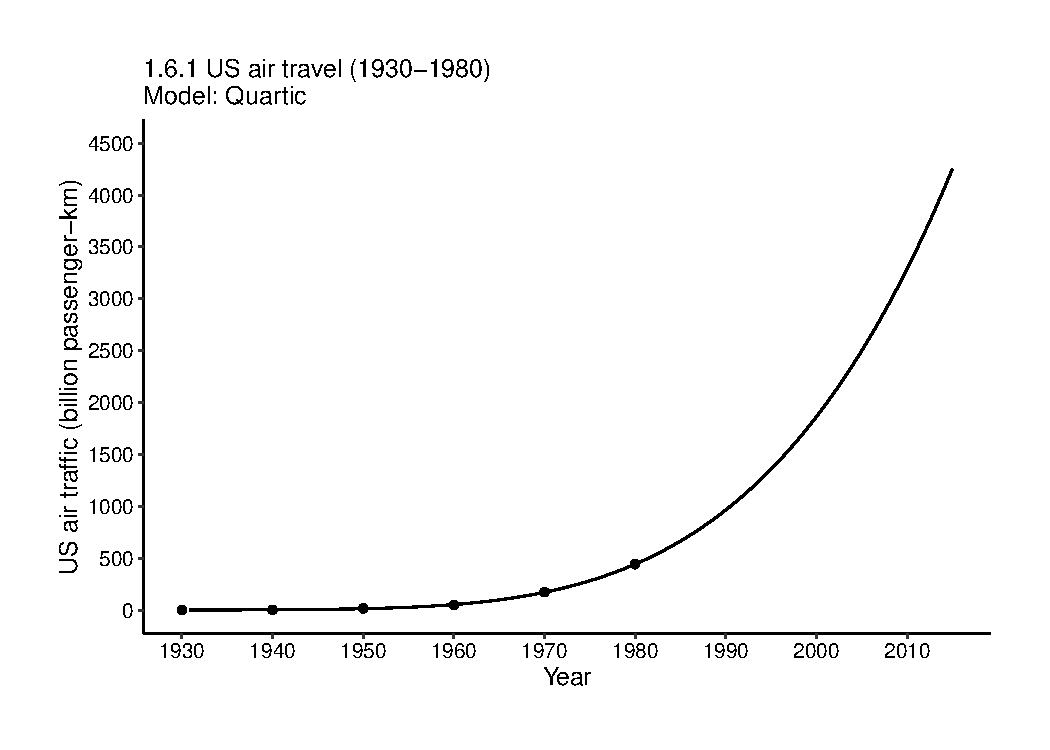
\includegraphics[width=\textwidth]{output/figs-ggplot/1.6.1.pdf}
\caption*{\textbf{Dataset 1.6.1} (p. 22). Prediction of growth of US air travel (in billions of passenger-kilometers) based on the period 1930-1980. The best fit is a quartic regression. Data from various annual reports by the International Civil Aviation Organization. }
\end{figure}
	
\clearpage
\begin{figure}[h]
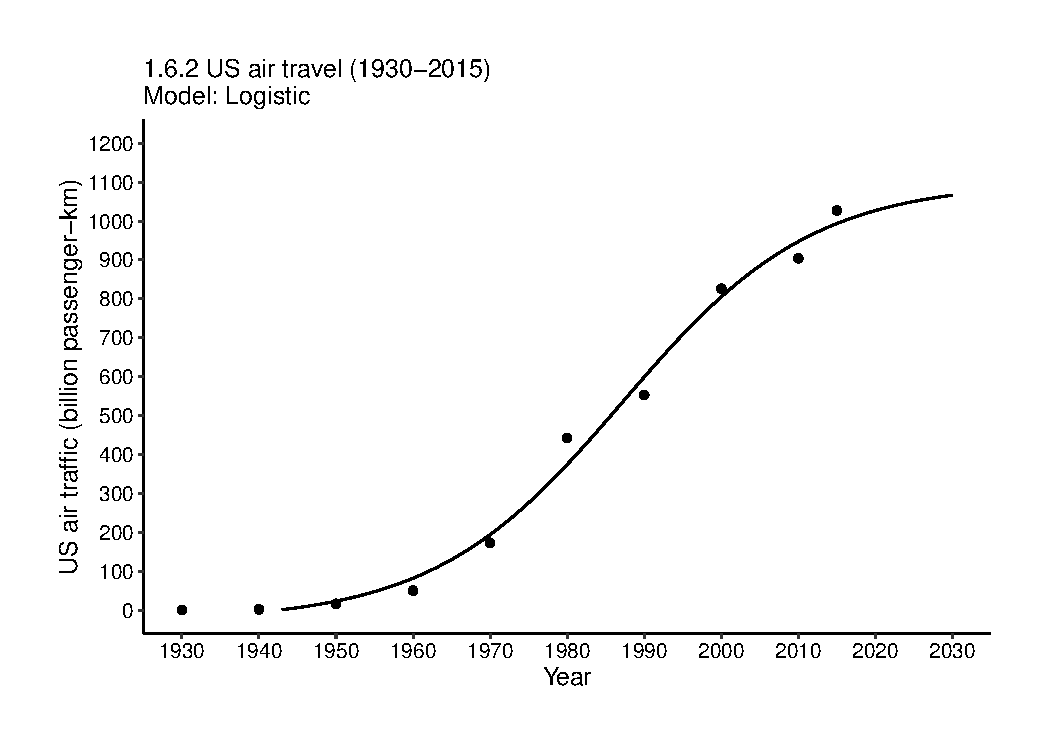
\includegraphics[width=\textwidth]{output/figs-ggplot/1.6.2.pdf}
\caption*{\textbf{Dataset 1.6.2} (p. 22). Prediction of growth of US air travel (in billions of passenger-kilometers) based on the period 1930-2015. The best fit is a logistic curve with the inflection year in 1987. Data from various annual reports by the International Civil Aviation Organization. }
\end{figure}
	
\clearpage
\begin{figure}[h]
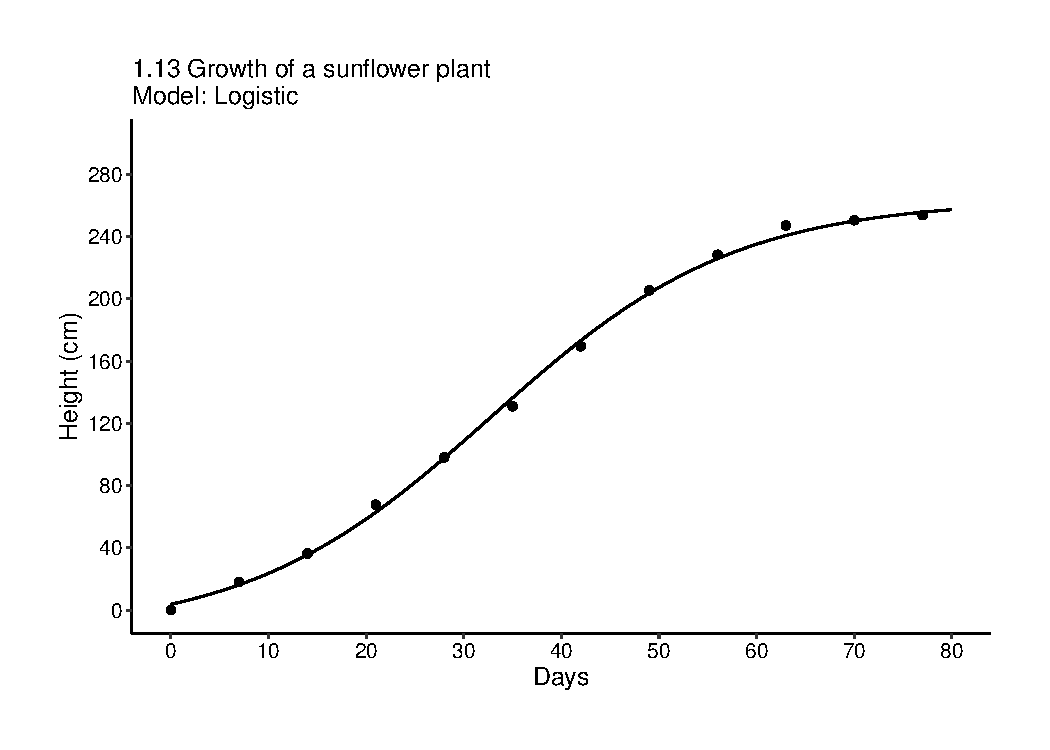
\includegraphics[width=\textwidth]{output/figs-ggplot/1.13.pdf}
\caption*{\textbf{Dataset 1.13} (p. 39). Logistic growth (inflection point at 37.1 days, asymptote at 292.9cm) of a sunflower plant plotted by Reed and Holland (1919). }
\end{figure}
	
\clearpage
\begin{figure}[h]
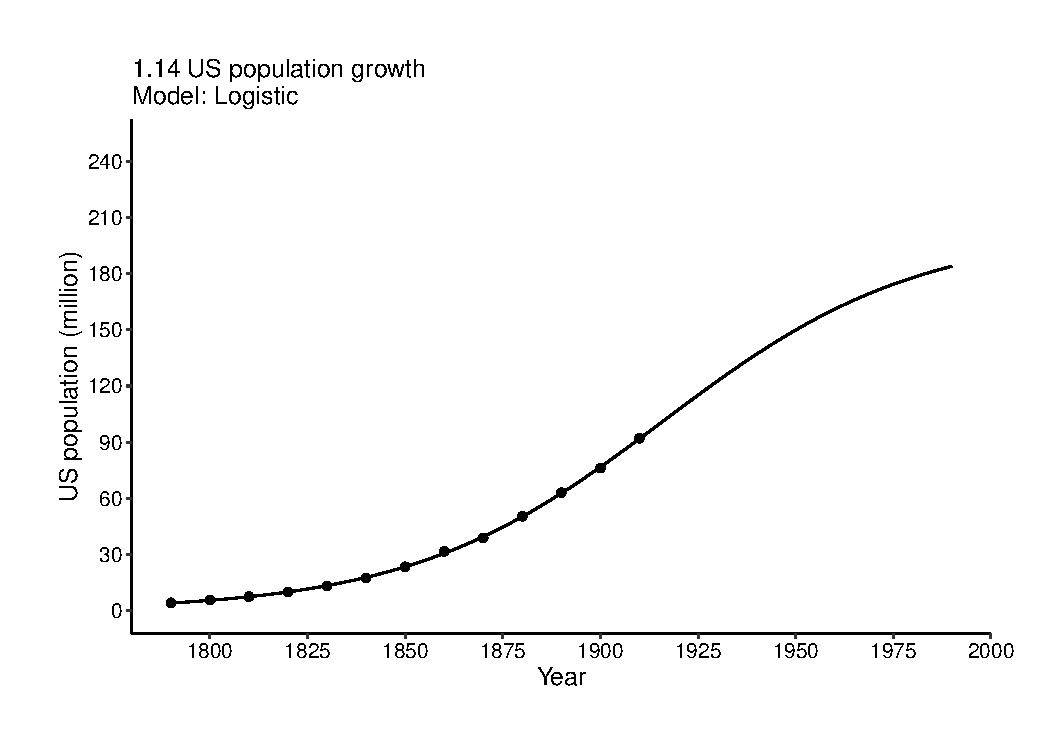
\includegraphics[width=\textwidth]{output/figs-ggplot/1.14.pdf}
\caption*{\textbf{Dataset 1.14} (p. 40). Forecast of US population growth based on the logistic curve (inflection point in 1919, asymptote at 197.3 million) fitted to decennial census data between 1790 and 1930. Data from Pearl and Reed (1920).}
\end{figure}
	
\clearpage
\begin{figure}[h]
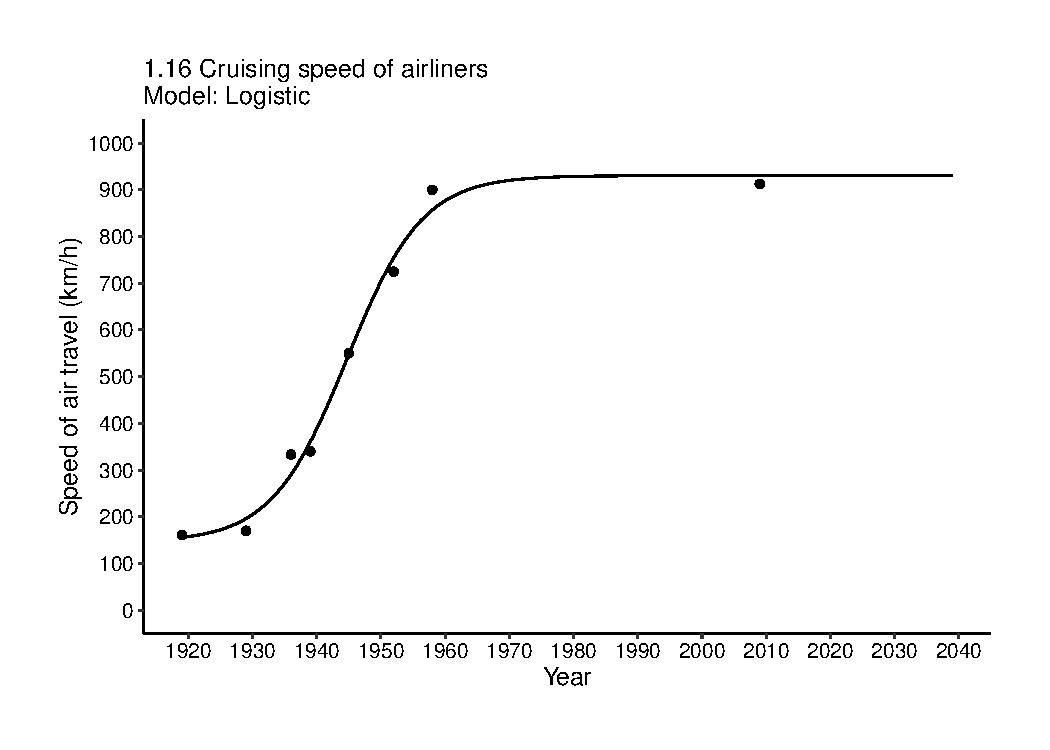
\includegraphics[width=\textwidth]{output/figs-ggplot/1.16.pdf}
\caption*{\textbf{Dataset 1.16} (p. 45). Logistic curve tracing the growth of cruising speed of commercial airliners 1919-2039 (inflection point in 1945, asymptotic cruising speed of 930.8 km/h). Plotted from data on speeds of specific airplanes, starting with KLM's de Havilland DH-16 in 1919 and ending with Boeing 787 in 2009. }
\end{figure}
	
\clearpage
\begin{figure}[h]
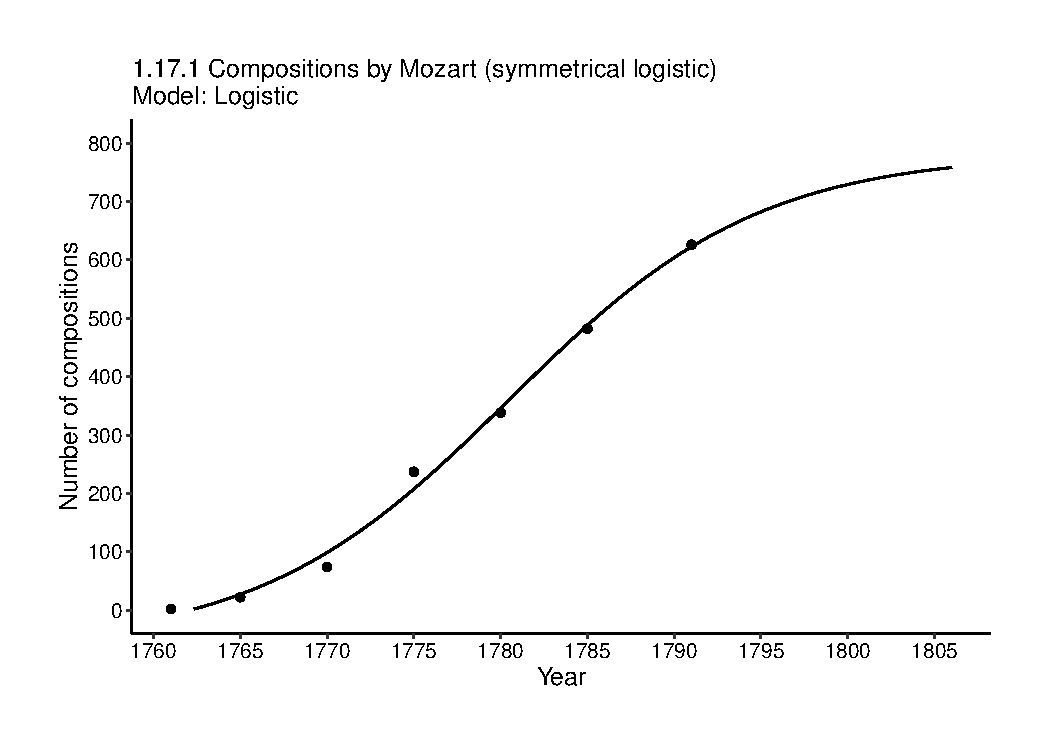
\includegraphics[width=\textwidth]{output/figs-ggplot/1.17.1.pdf}
\caption*{\textbf{Dataset 1.17.1} (p. 47). Fitting Mozart's oeuvre into growth curves: symmetrical (a)and asymmetrical (b) logistic functions and quadratic (c) and quartic (d) regression all have high degrees of fit ($R^2=0.99$) but predict substantially different long-term outcomes for the year 1806 when Mozart (who died in 1791) would have been 50 years old. Compositions by date listed in Giegling et al. (1964).}
\end{figure}
	
\clearpage
\begin{figure}[h]
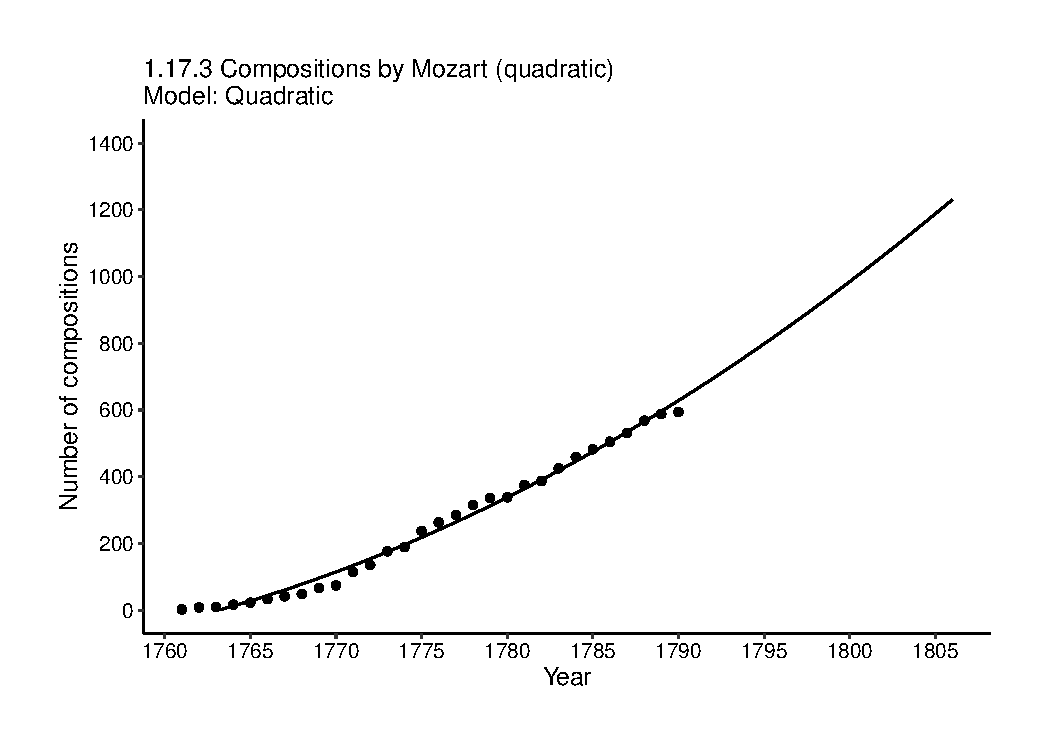
\includegraphics[width=\textwidth]{output/figs-ggplot/1.17.3.pdf}
\caption*{\textbf{Dataset 1.17.3} (p. 47). Fitting Mozart's oeuvre into growth curves: symmetrical (a)and asymmetrical (b) logistic functions and quadratic (c) and quartic (d) regression all have high degrees of fit ($R^2=0.99$) but predict substantially different long-term outcomes for the year 1806 when Mozart (who died in 1791) would have been 50 years old. Compositions by date listed in Giegling et al. (1964).}
\end{figure}
	
\clearpage
\begin{figure}[h]
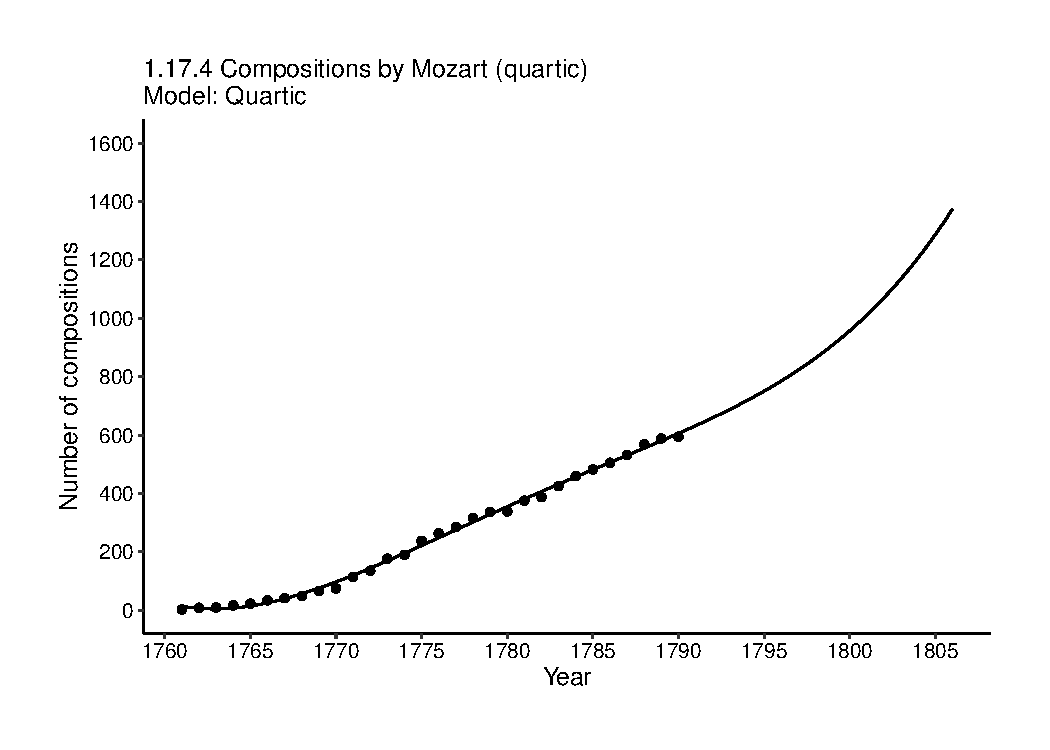
\includegraphics[width=\textwidth]{output/figs-ggplot/1.17.4.pdf}
\caption*{\textbf{Dataset 1.17.4} (p. 47). Fitting Mozart's oeuvre into growth curves: symmetrical (a)and asymmetrical (b) logistic functions and quadratic (c) and quartic (d) regression all have high degrees of fit ($R^2=0.99$) but predict substantially different long-term outcomes for the year 1806 when Mozart (who died in 1791) would have been 50 years old. Compositions by date listed in Giegling et al. (1964).}
\end{figure}
	
\clearpage
\begin{figure}[h]
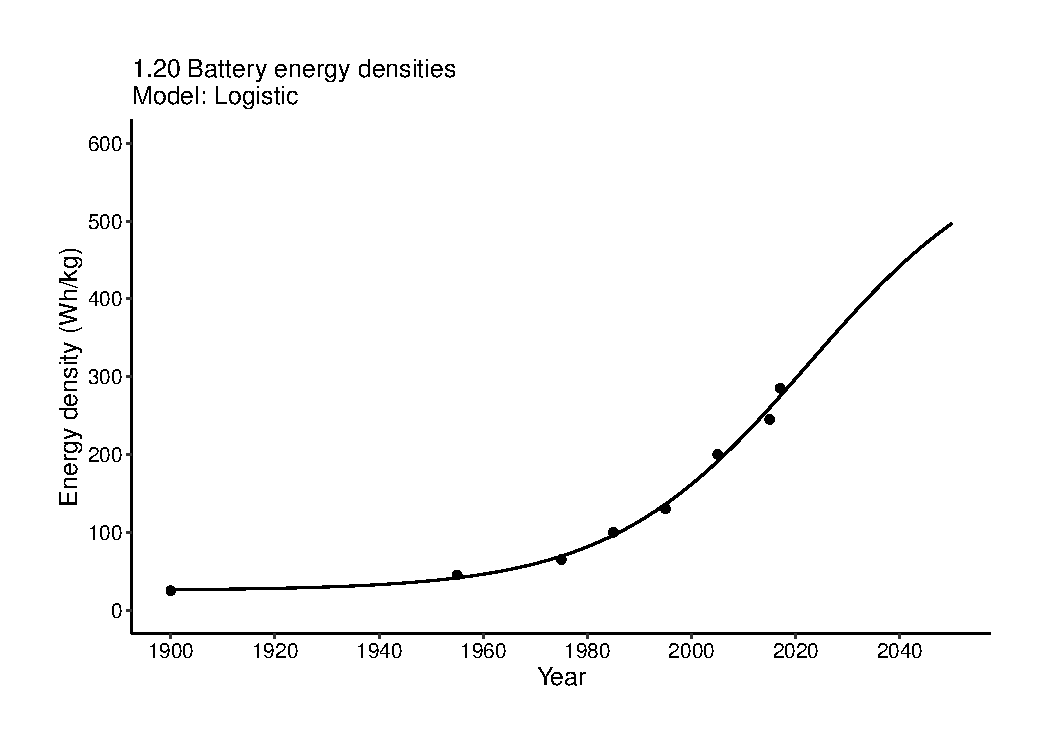
\includegraphics[width=\textwidth]{output/figs-ggplot/1.20.pdf}
\caption*{\textbf{Dataset 1.20} (p. 51). Logistic growth trajectory (inflection point in 2024, asymptote at 625.5 Wh/kg) of battery energy densities, 1900-2017. Plotted from data in Zu and Li (2011) and from subsequent news reports. }
\end{figure}
	
\clearpage
\begin{figure}[h]
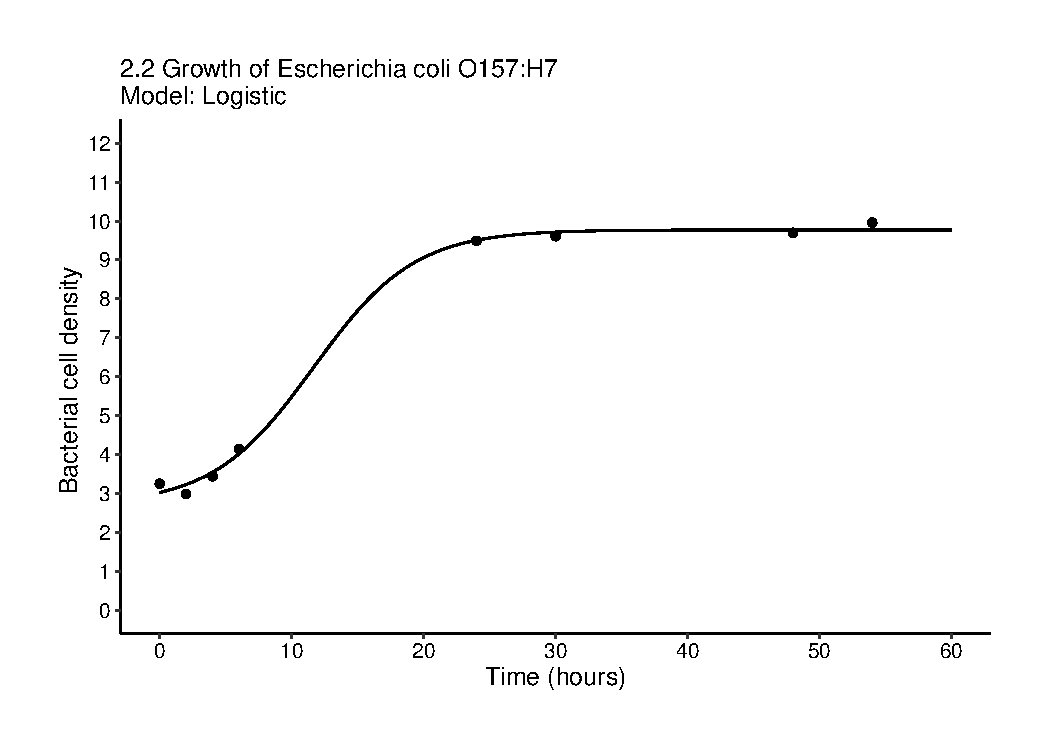
\includegraphics[width=\textwidth]{output/figs-ggplot/2.2.pdf}
\caption*{\textbf{Dataset 2.2} (p. 80). Logistic growth of Escherichia coli O157:H7. Plotted from data in Buchanan et al. (1997).}
\end{figure}
	
\clearpage
\begin{figure}[h]
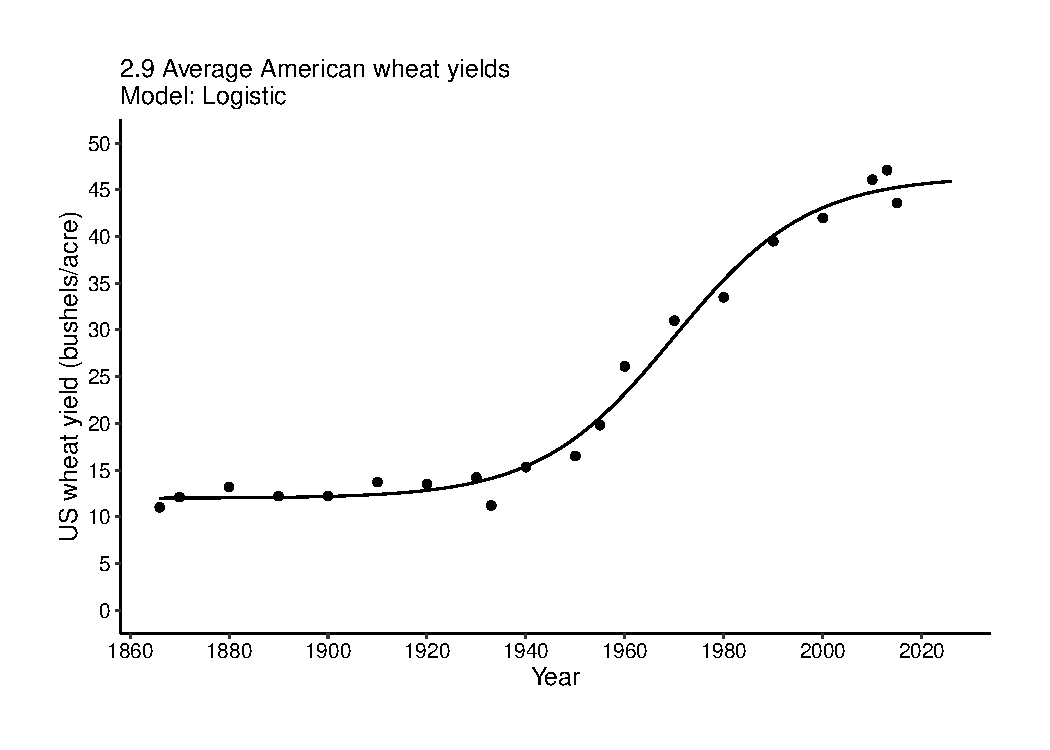
\includegraphics[width=\textwidth]{output/figs-ggplot/2.9.pdf}
\caption*{\textbf{Dataset 2.9} (p. 119). Logistic growth (inflection point in 1970, asymptote at 46.5 bushels/acre) of average American wheat yields, 1866-2015. Data from USDA (2017a).}
\end{figure}
	
\clearpage
\begin{figure}[h]
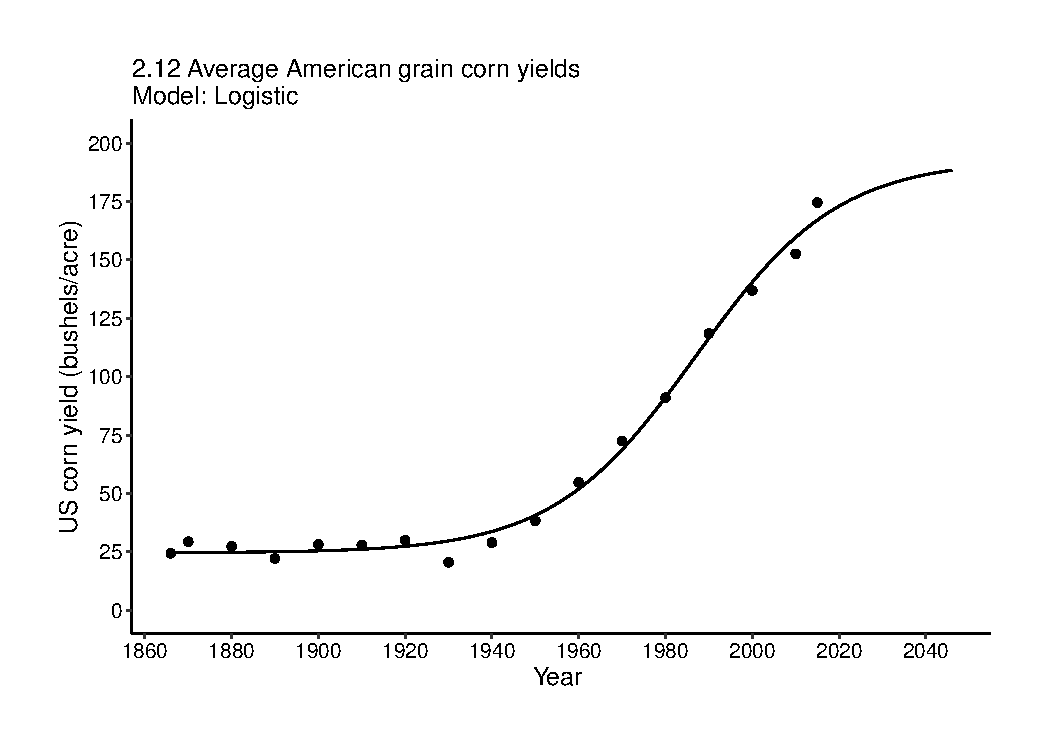
\includegraphics[width=\textwidth]{output/figs-ggplot/2.12.pdf}
\caption*{\textbf{Dataset 2.12} (p. 124). Logistic growth trajectory (inflection point in 1988, asymptote at 194.1 bushels/acre) of average American grain corn yields, 1866-2015. Data from USDA (2017a).}
\end{figure}
	
\clearpage
\begin{figure}[h]
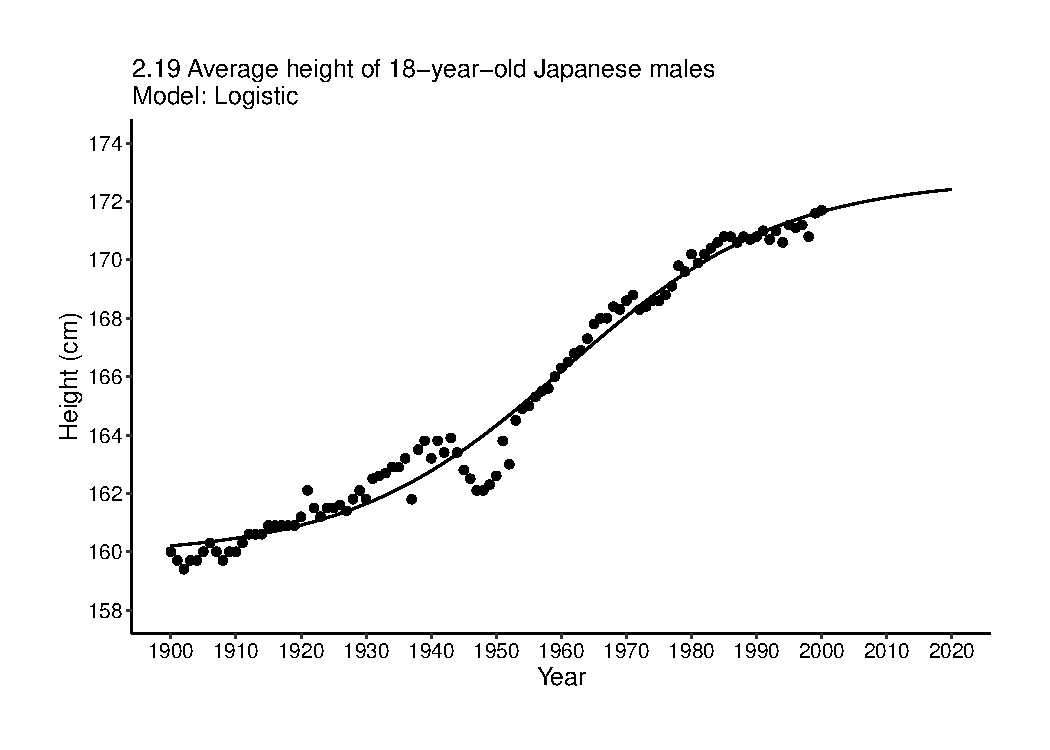
\includegraphics[width=\textwidth]{output/figs-ggplot/2.19.pdf}
\caption*{\textbf{Dataset 2.19} (p. 166). Average height of 18-year-old Japanese males, 1900-2020. Plotted from data in SB (1996). Logistic curve has $R^2$ of 0.98, inflection point in 1961, and asymptote height is 172.8 cm. }
\end{figure}
	
\clearpage
\begin{figure}[h]
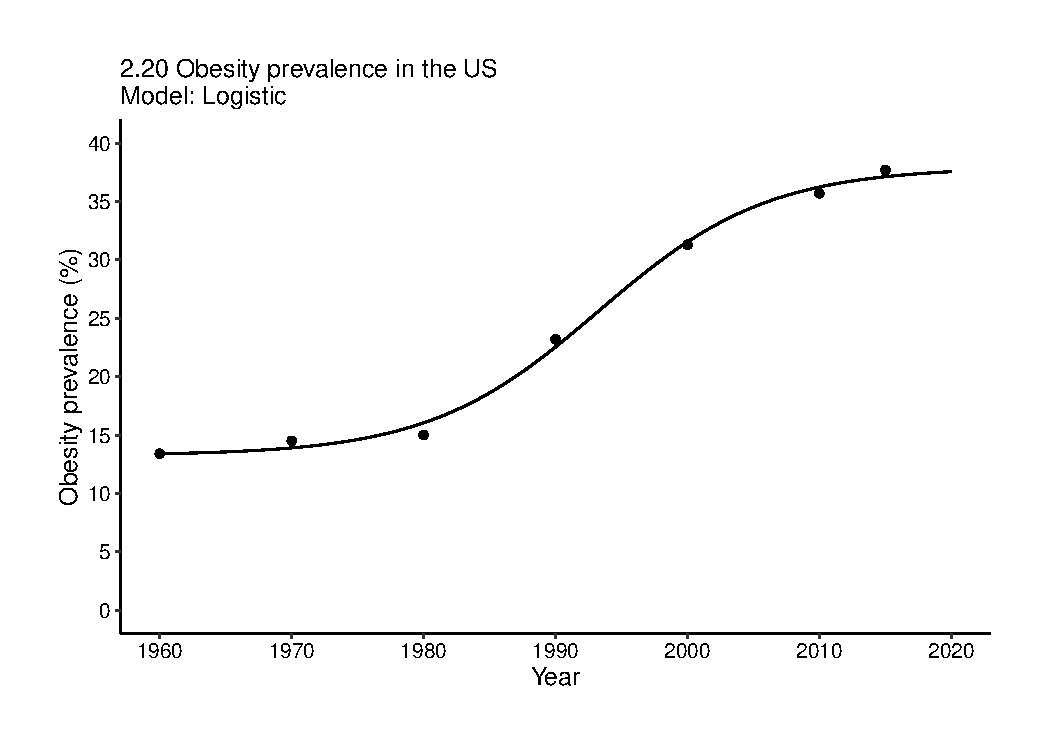
\includegraphics[width=\textwidth]{output/figs-ggplot/2.20.pdf}
\caption*{\textbf{Dataset 2.20} (p. 170). Growing prevalence of obesity in the US. Data from Ogden et al. (2012) and The State of Obesity (2012). The logistic curve had its inflection point in 1993 and its asymptote is at 37.5\% of the total population.}
\end{figure}
	
\clearpage
\begin{figure}[h]
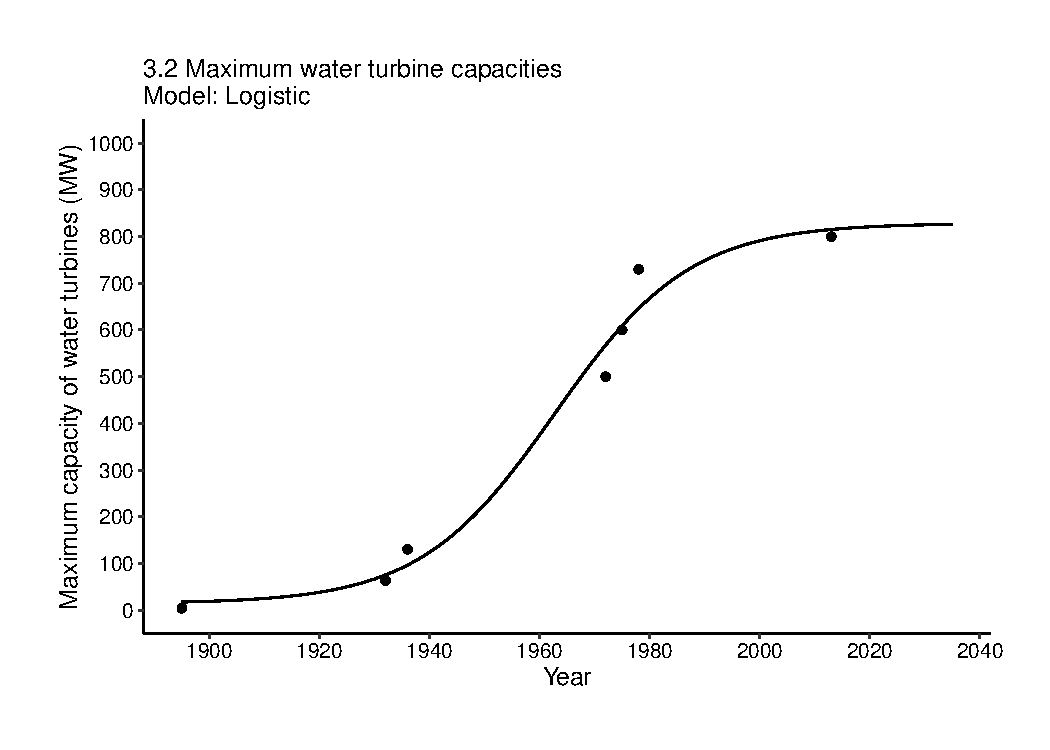
\includegraphics[width=\textwidth]{output/figs-ggplot/3.2.pdf}
\caption*{\textbf{Dataset 3.2} (p. 181). Logistic growth of maximum water turbine capacities since 1895; inflection point was in 1963. Data from Smil (2008) and ICOLD (2017).}
\end{figure}
	
\clearpage
\begin{figure}[h]
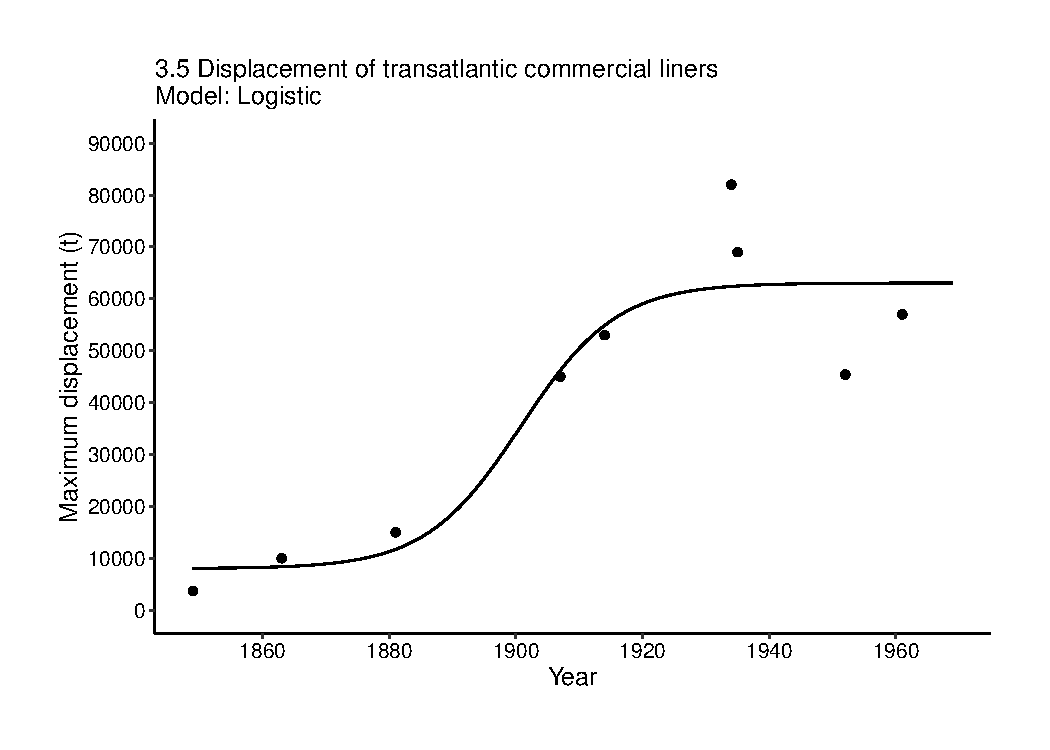
\includegraphics[width=\textwidth]{output/figs-ggplot/3.5.pdf}
\caption*{\textbf{Dataset 3.5} (p. 191). Logistic curve of the maximum displacement of transatlantic commercial liners, 1849-1961 (Smil 2017a).}
\end{figure}
	
\clearpage
\begin{figure}[h]
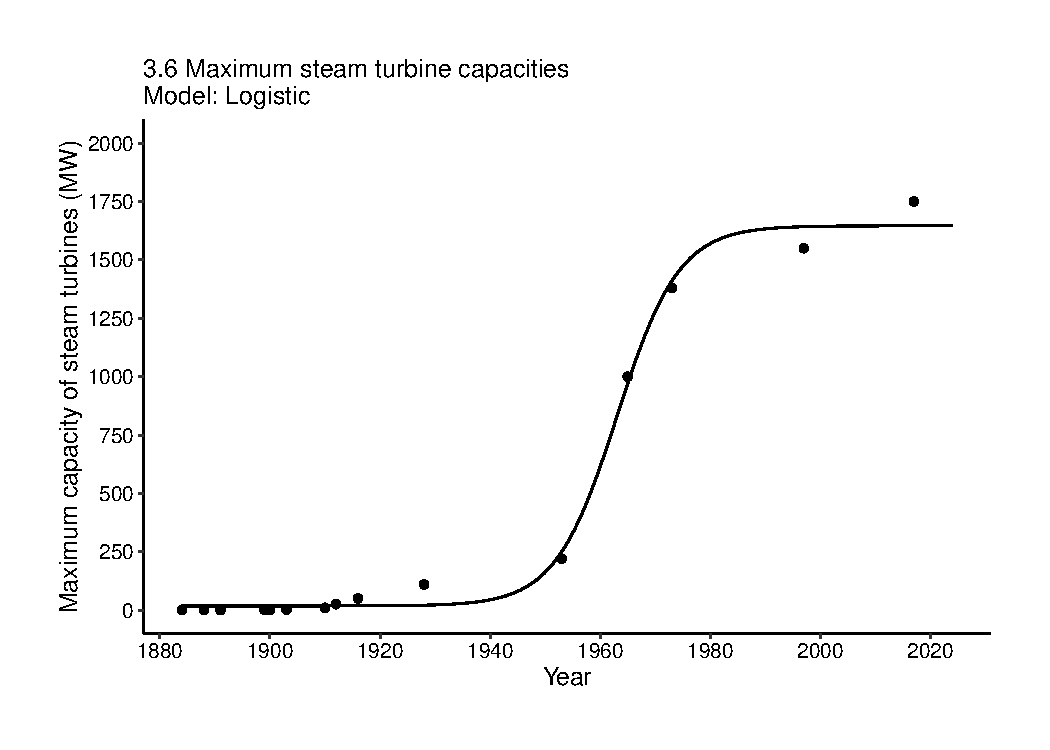
\includegraphics[width=\textwidth]{output/figs-ggplot/3.6.pdf}
\caption*{\textbf{Dataset 3.6} (p. 195). Growth of maximum steam turbine capacities since 1884. Five-parameter [sic] logistic curve, inflection year in 1954, asymptote has been already reached. Data from Smil (2003, 2017a).}
\end{figure}
	
\clearpage
\begin{figure}[h]
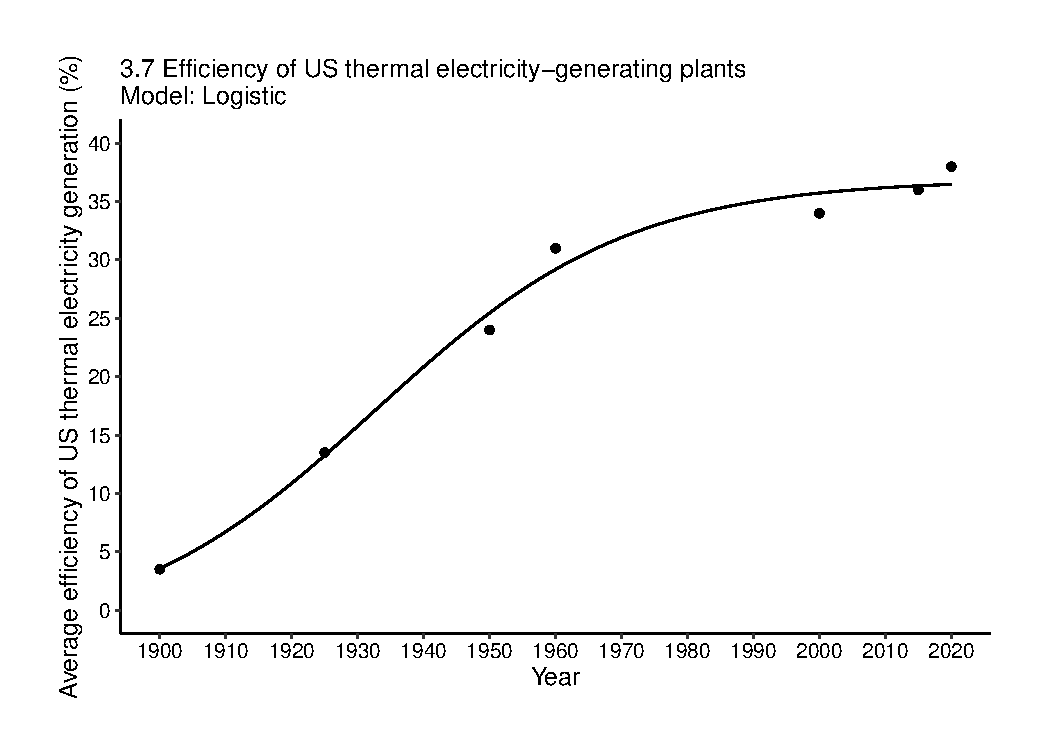
\includegraphics[width=\textwidth]{output/figs-ggplot/3.7.pdf}
\caption*{\textbf{Dataset 3.7} (p. 196). Logistic growth (inflection year in 1933, asymptote at 36.9\%) of average efficiency of US thermal electricity-generating plants. Data from Schurr and Netschert (1960) and USEIA (2016).}
\end{figure}
	
\clearpage
\begin{figure}[h]
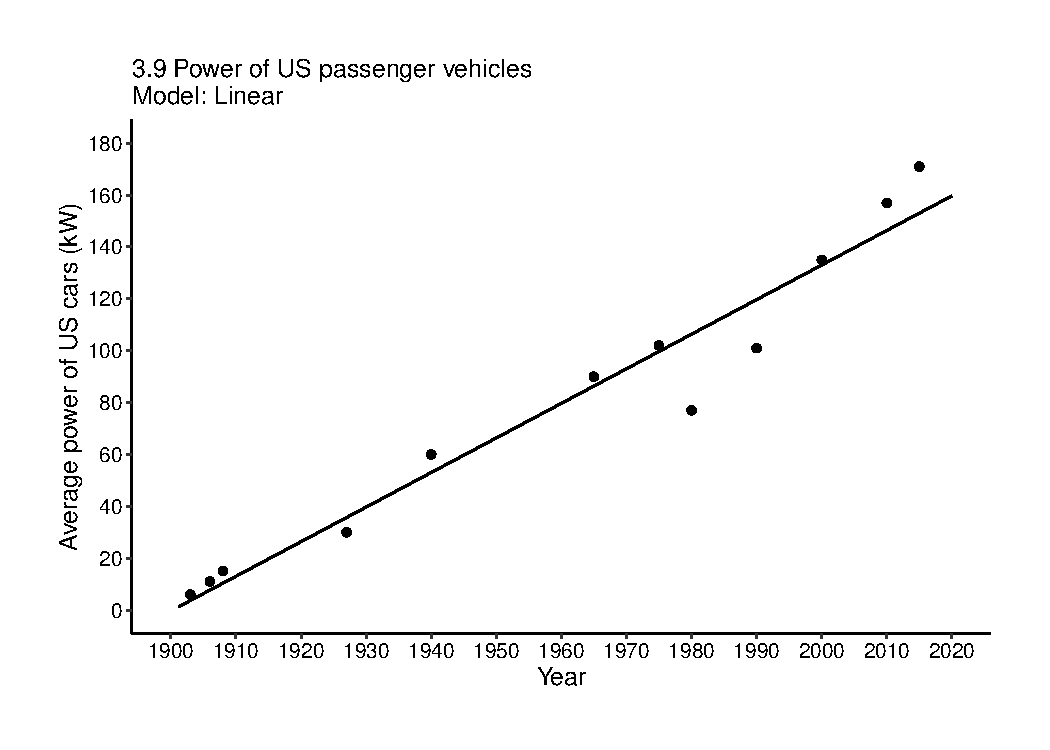
\includegraphics[width=\textwidth]{output/figs-ggplot/3.9.pdf}
\caption*{\textbf{Dataset 3.9} (p. 200). Linear growth of average power of US passenger vehicles, 1903-2020. Data from Smil (2014b) and USEPA (2016b).}
\end{figure}
	
\clearpage
\begin{figure}[h]
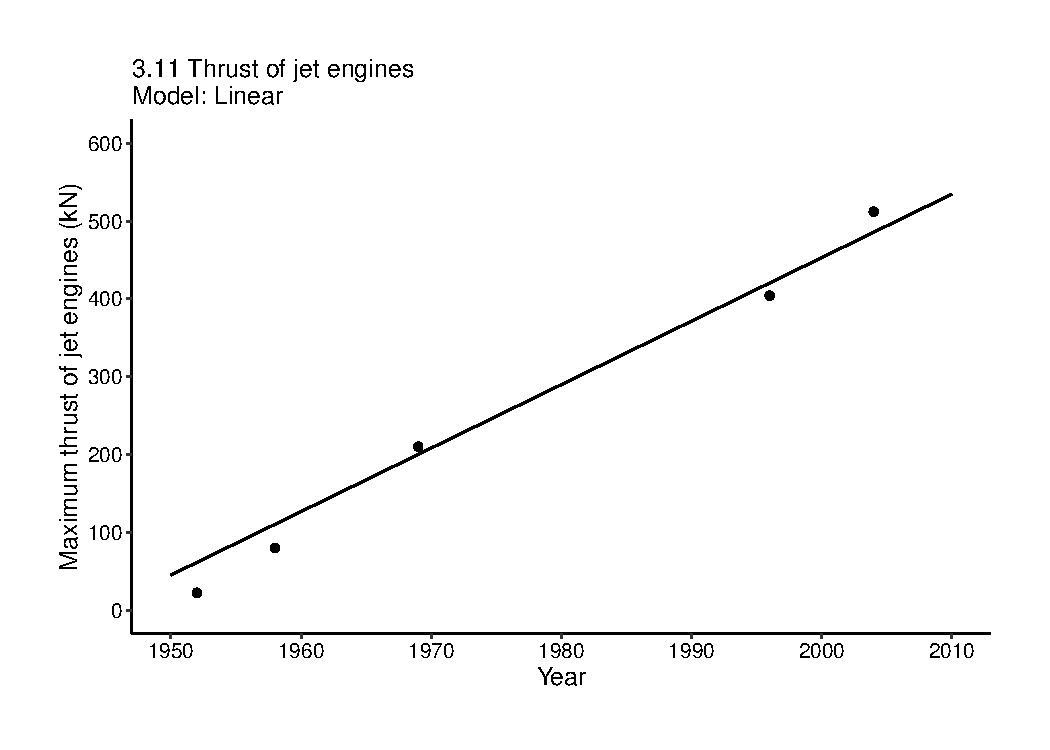
\includegraphics[width=\textwidth]{output/figs-ggplot/3.11.pdf}
\caption*{\textbf{Dataset 3.11} (p. 209). Linear fit of the maximum thrust of jet engines. Data from Smil (2010b).}
\end{figure}
	
\clearpage
\begin{figure}[h]
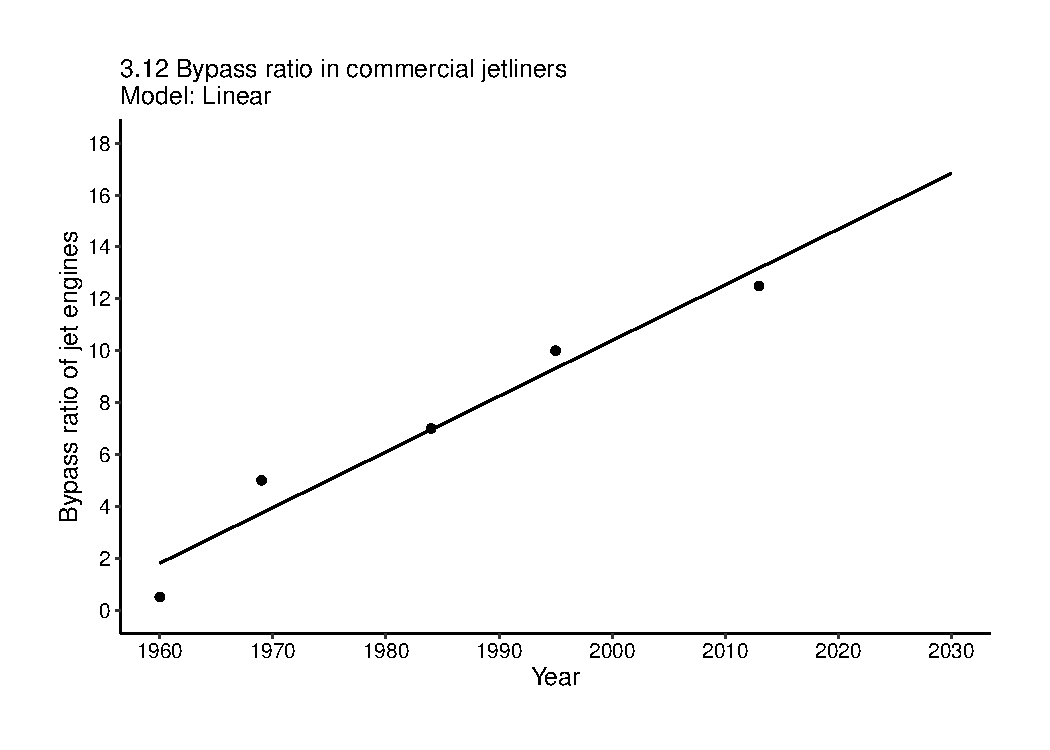
\includegraphics[width=\textwidth]{output/figs-ggplot/3.12.pdf}
\caption*{\textbf{Dataset 3.12} (p. 210). Evolution of the bypass ratio in commercial jetliners. Data from specifications for GE, P\&W, and Rolls-Royce engines and from Ballal and Zelina (2003). Maximum ratios have seen linear growth that averaged about 2.2 units per decade.}
\end{figure}
	
\clearpage
\begin{figure}[h]
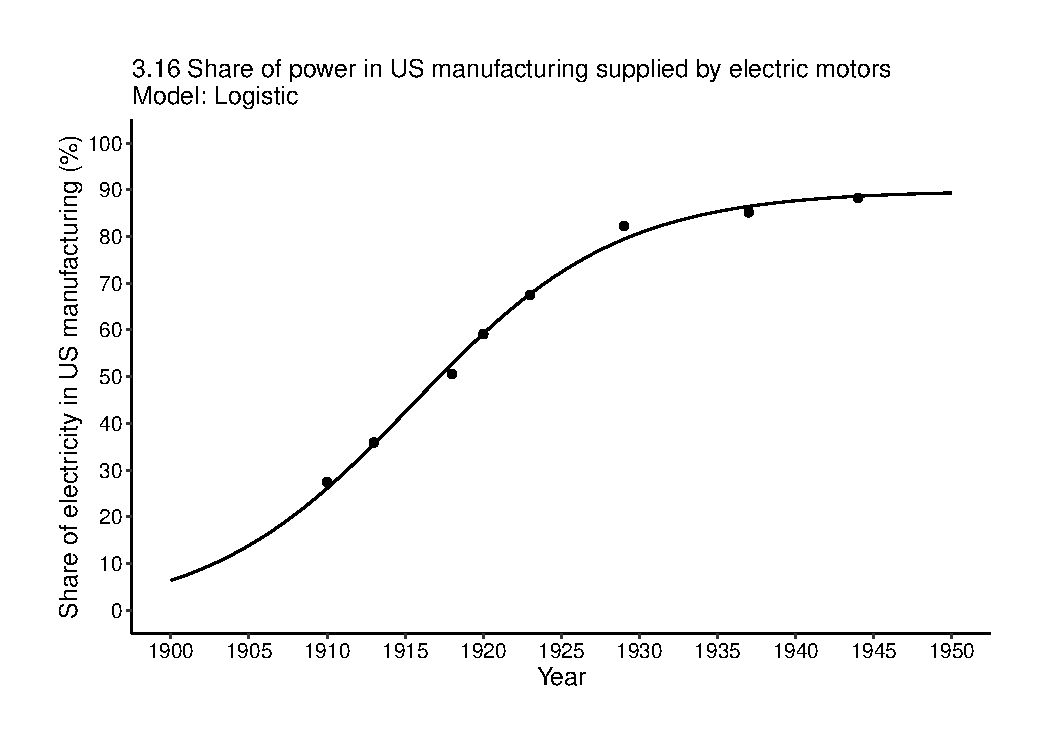
\includegraphics[width=\textwidth]{output/figs-ggplot/3.16.pdf}
\caption*{\textbf{Dataset 3.16} (p. 221). Logistic fit (inflection point in 1916, asymptote of 89.9\%) of the share of power in US manufacturing supplied by electric motors, 1909-1950. Data from Daugherty (1927) and Schurr et al. (1990).}
\end{figure}
	
\clearpage
\begin{figure}[h]
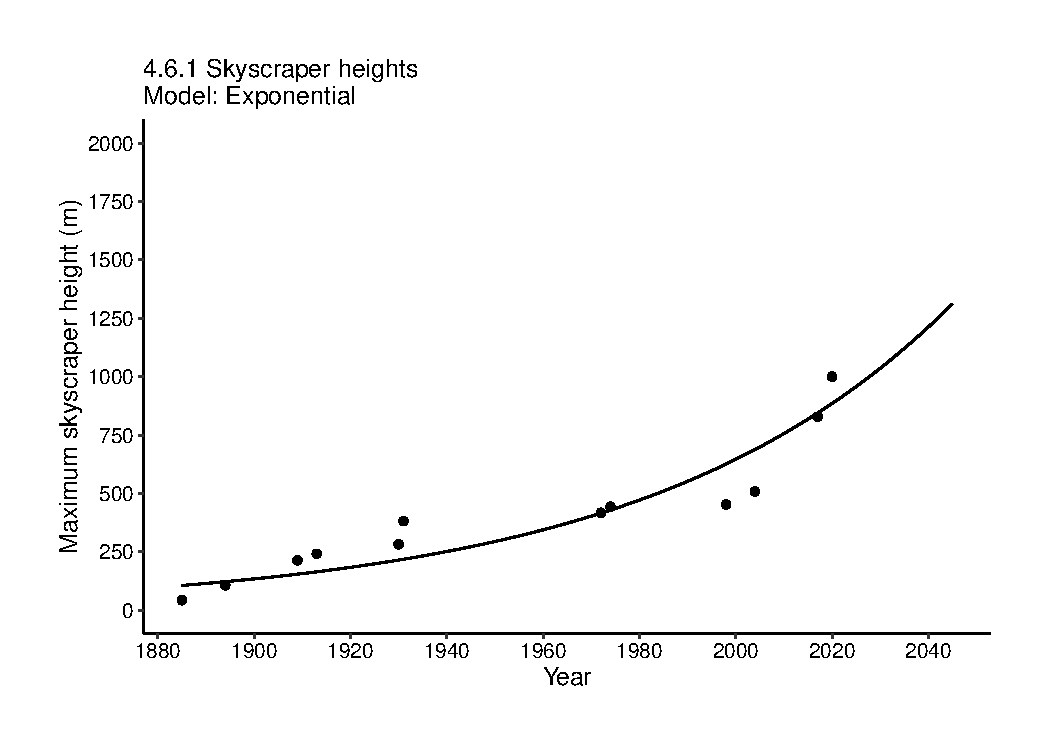
\includegraphics[width=\textwidth]{output/figs-ggplot/4.6.1.pdf}
\caption*{\textbf{Dataset 4.6.1} (p. 245). Logistic curve of the growth of maximum skyscraper height. Data from Landau and Condit (1996) and Skyscraper Center (2017).}
\end{figure}
	
\clearpage
\begin{figure}[h]
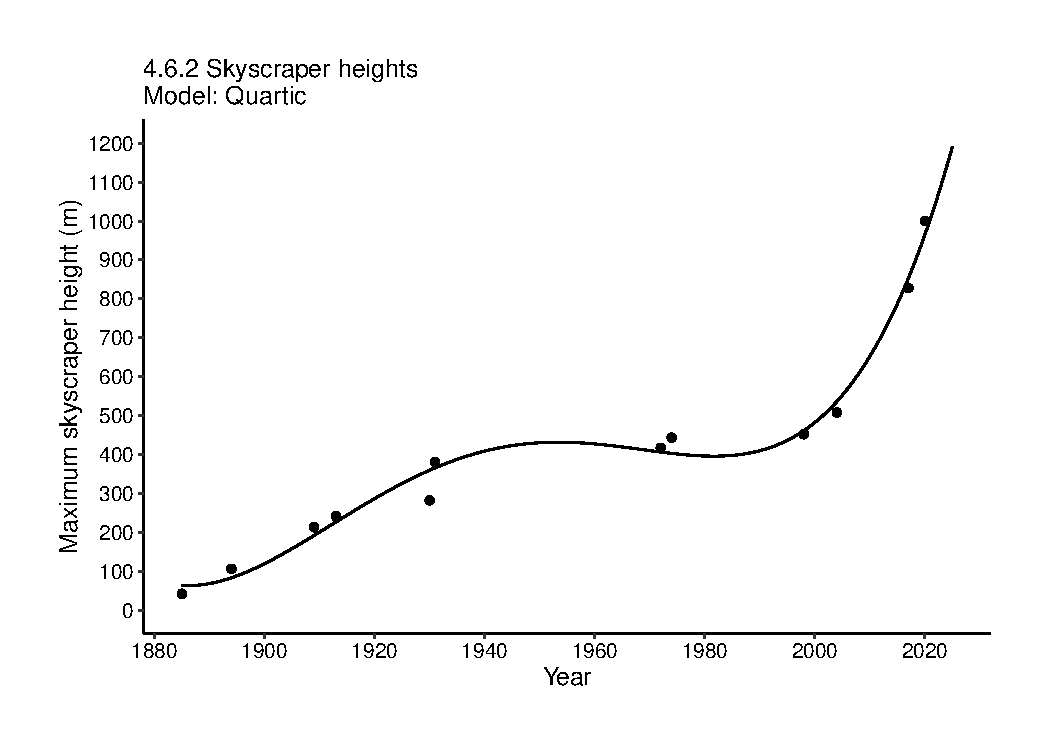
\includegraphics[width=\textwidth]{output/figs-ggplot/4.6.2.pdf}
\caption*{\textbf{Dataset 4.6.2} (p. 245). Polynomial regression of the growth of maximum skyscraper height. Data from Landau and Condit (1996) and Skyscraper Center (2017). }
\end{figure}
	
\clearpage
\begin{figure}[h]
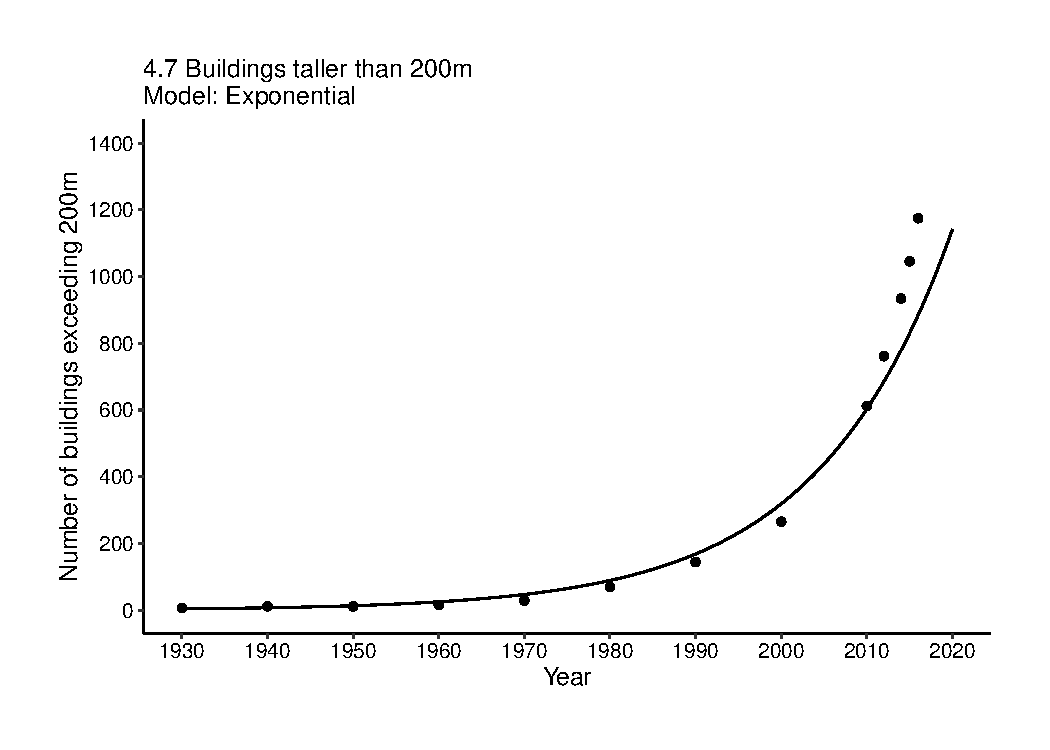
\includegraphics[width=\textwidth]{output/figs-ggplot/4.7.pdf}
\caption*{\textbf{Dataset 4.7} (p. 247). Growth of the total number of buildings taller than 200m. Logistic curve in its early stage of ascent. Data from Emporis (2017).}
\end{figure}
	
\clearpage
\begin{figure}[h]
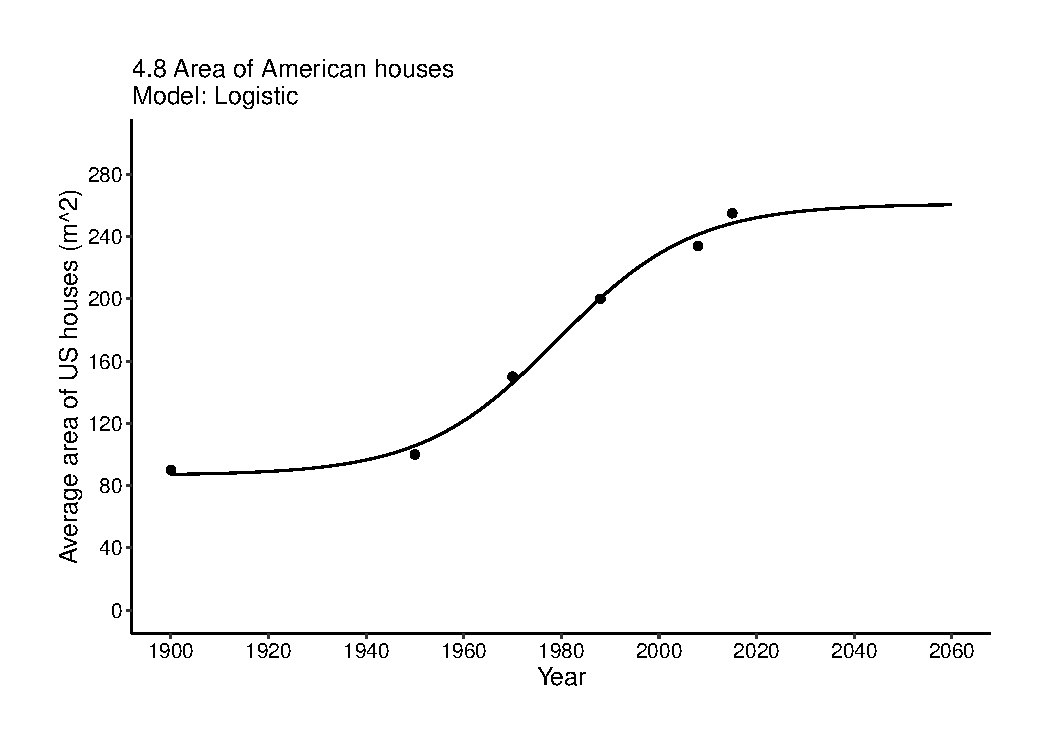
\includegraphics[width=\textwidth]{output/figs-ggplot/4.8.pdf}
\caption*{\textbf{Dataset 4.8} (p. 250). Growth of the average area of American houses since 1900. Logistic curve had the inflection year in 1979 and its asymptote is about 260 m$^2$. Data from Wilson and Boehland (2005) and USCB (2016a).}
\end{figure}
	
\clearpage
\begin{figure}[h]
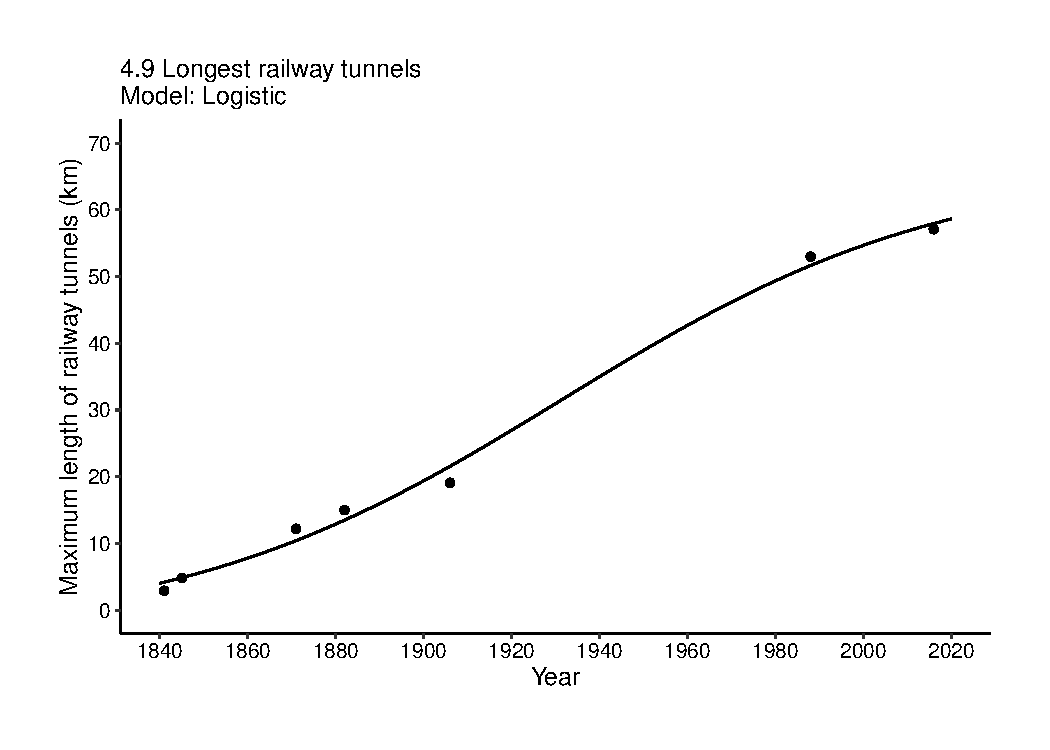
\includegraphics[width=\textwidth]{output/figs-ggplot/4.9.pdf}
\caption*{\textbf{Dataset 4.9} (p. 256). Growth of the longest railway tunnels, 1840-2020. Data mostly from Beaver (1972) and Onoda (2015).}
\end{figure}
	
\clearpage
\begin{figure}[h]
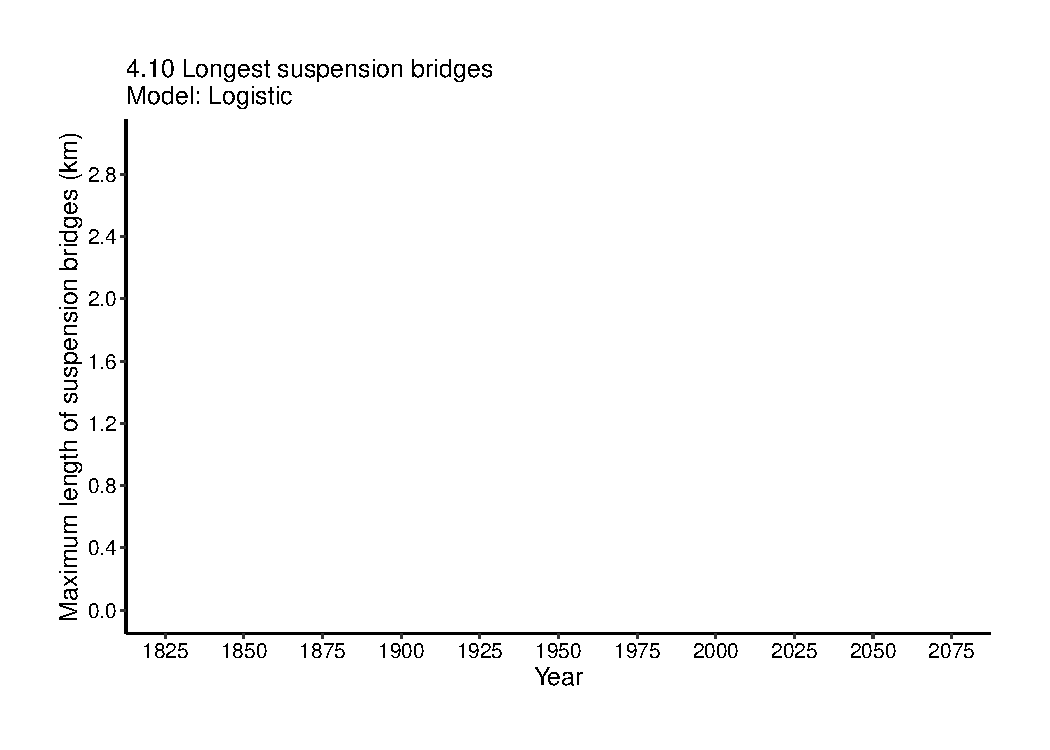
\includegraphics[width=\textwidth]{output/figs-ggplot/4.10.pdf}
\caption*{\textbf{Dataset 4.10} (p. 258). Growth of the longest suspension bridges since 1825. Data mostly from History of Bridges (2017).}
\end{figure}
	
\clearpage
\begin{figure}[h]
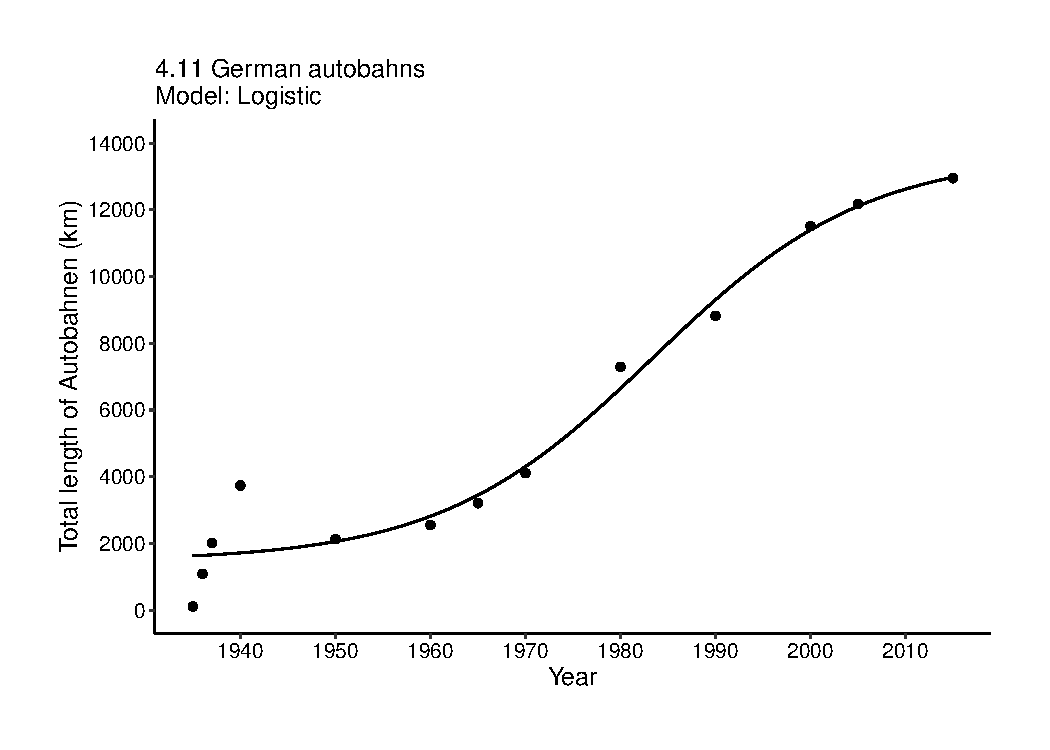
\includegraphics[width=\textwidth]{output/figs-ggplot/4.11.pdf}
\caption*{\textbf{Dataset 4.11} (p. 260). Growth curve of German Autobahnen, 1935-2015. Data from Zeller (2007) and Bundesamt für Statistik.}
\end{figure}
	
\clearpage
\begin{figure}[h]
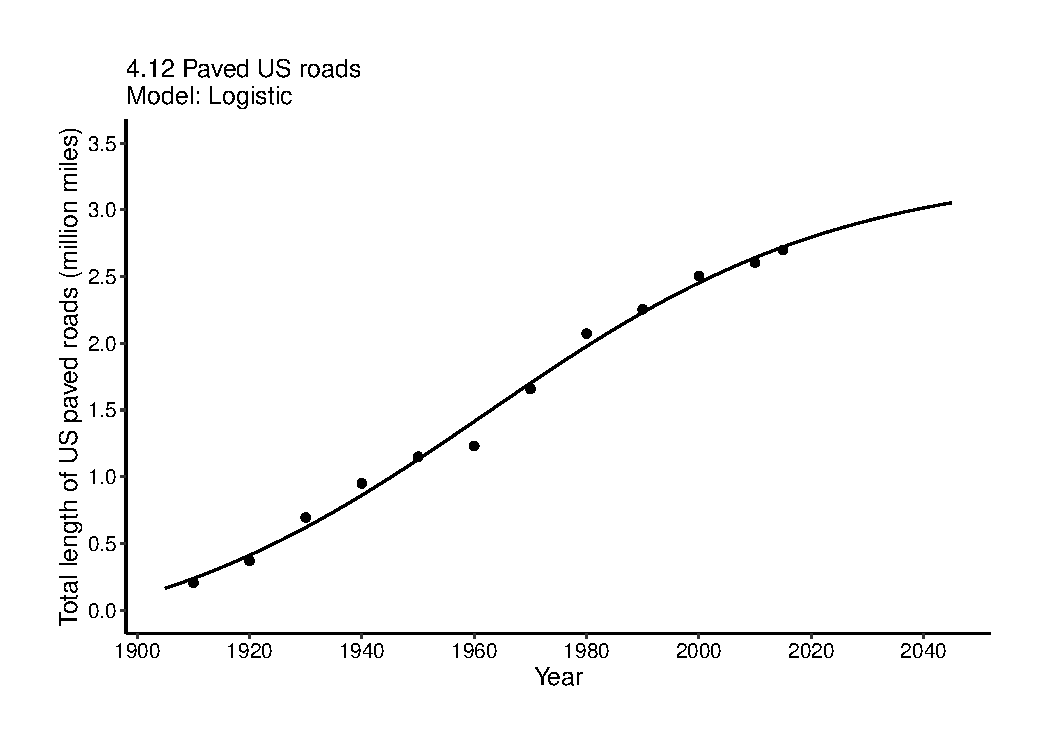
\includegraphics[width=\textwidth]{output/figs-ggplot/4.12.pdf}
\caption*{\textbf{Dataset 4.12} (p. 261). Growth of the total length of paved US roads since 1905. Plotted from data in USBC (1975) and subsequent volumes of US Statistical Abstract.}
\end{figure}
	
\clearpage
\begin{figure}[h]
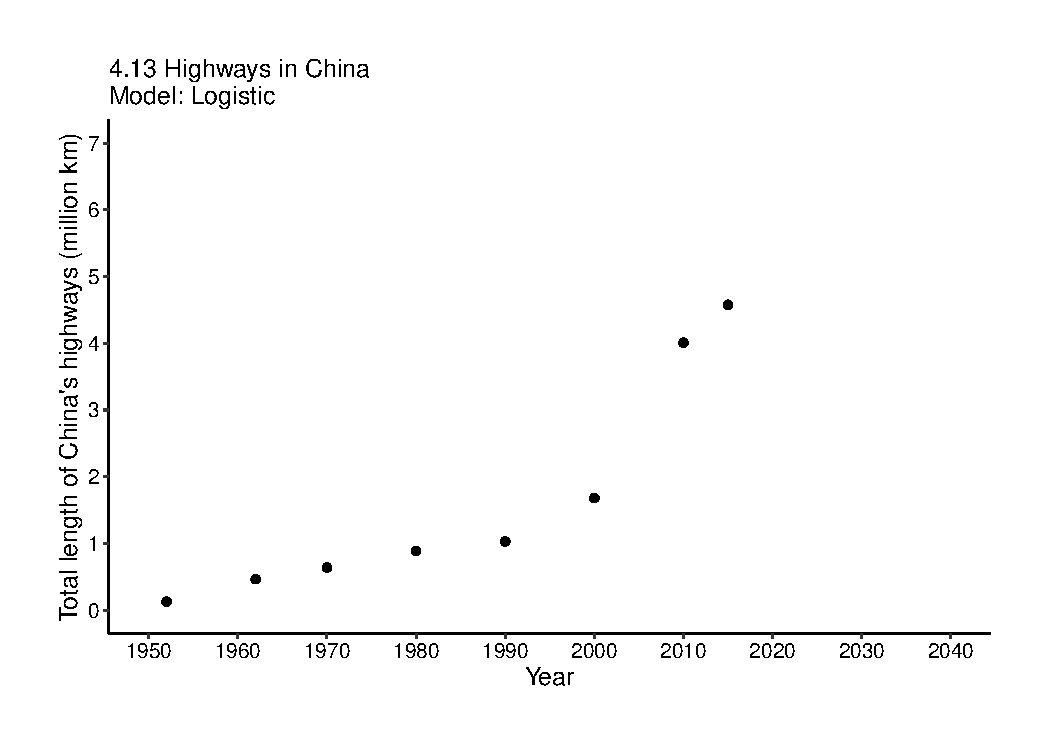
\includegraphics[width=\textwidth]{output/figs-ggplot/4.13.pdf}
\caption*{\textbf{Dataset 4.13} (p. 262). Growth of the total length of highways in China. Logistic curve with the inflection point in 2007 and asymptote about 30\% above the 2015 total. Data from NBS (2000, 2016).}
\end{figure}
	
\clearpage
\begin{figure}[h]
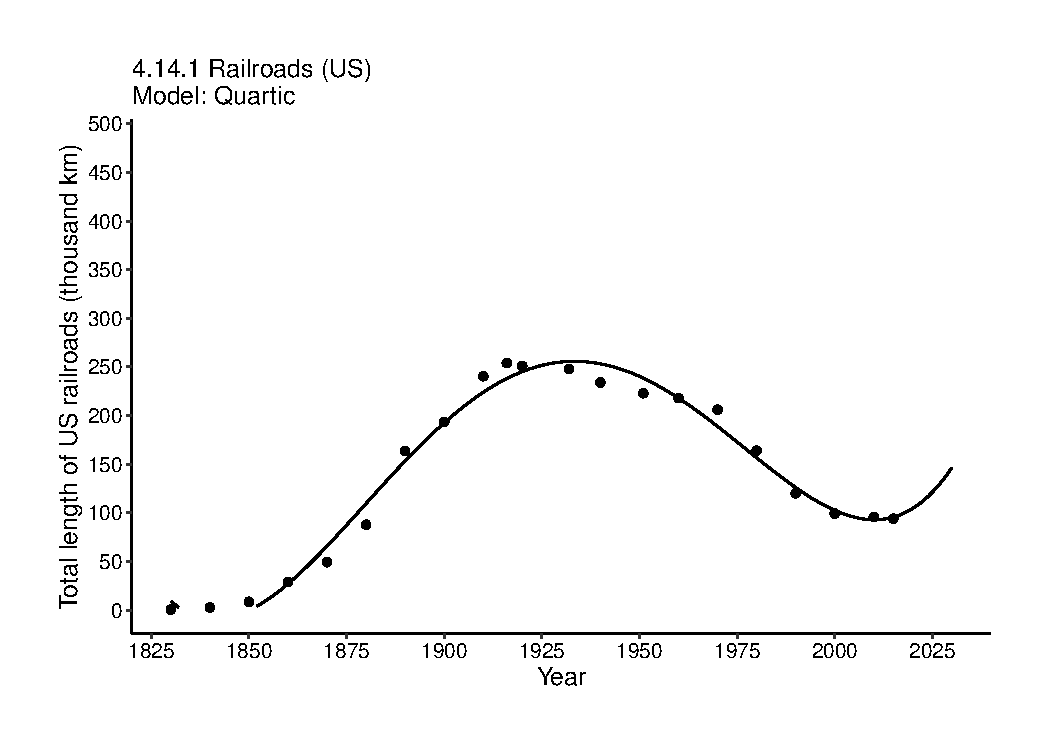
\includegraphics[width=\textwidth]{output/figs-ggplot/4.14.1.pdf}
\caption*{\textbf{Dataset 4.14.1} (p. 263). Growth curves of the total length of railroads in the US. Plotted from data in Mitchell (1998).}
\end{figure}
	
\clearpage
\begin{figure}[h]
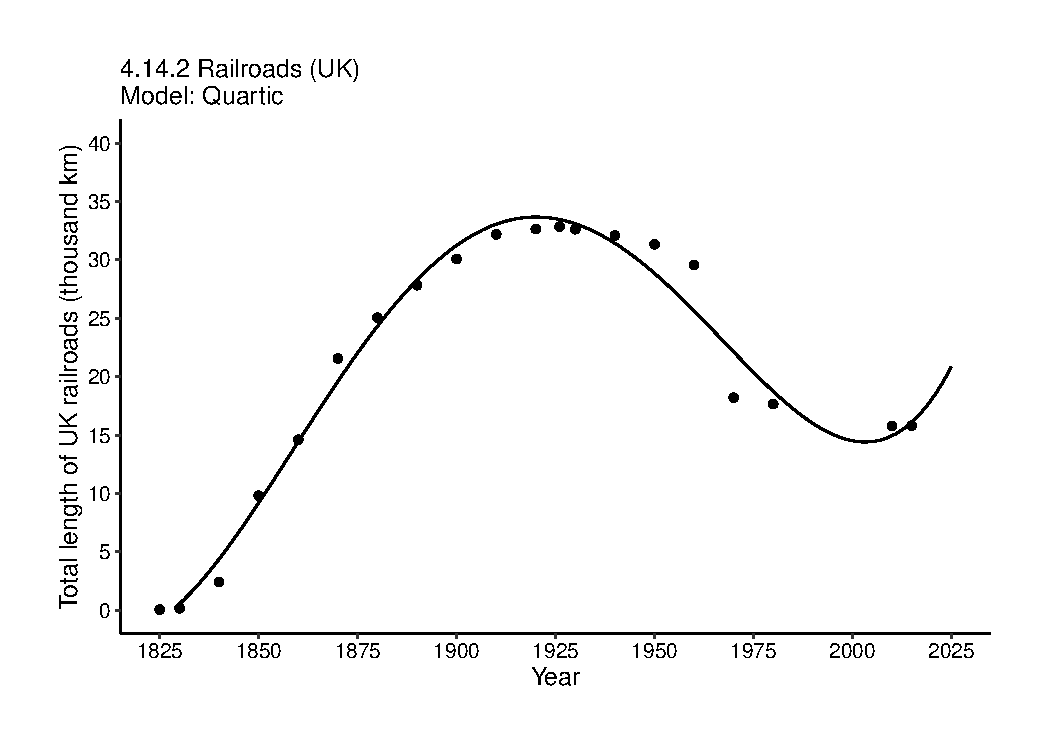
\includegraphics[width=\textwidth]{output/figs-ggplot/4.14.2.pdf}
\caption*{\textbf{Dataset 4.14.2} (p. 263). Growth curves of the total length of railroads in the UK. Plotted from data in Mitchell (1998).}
\end{figure}
	
\clearpage
\begin{figure}[h]
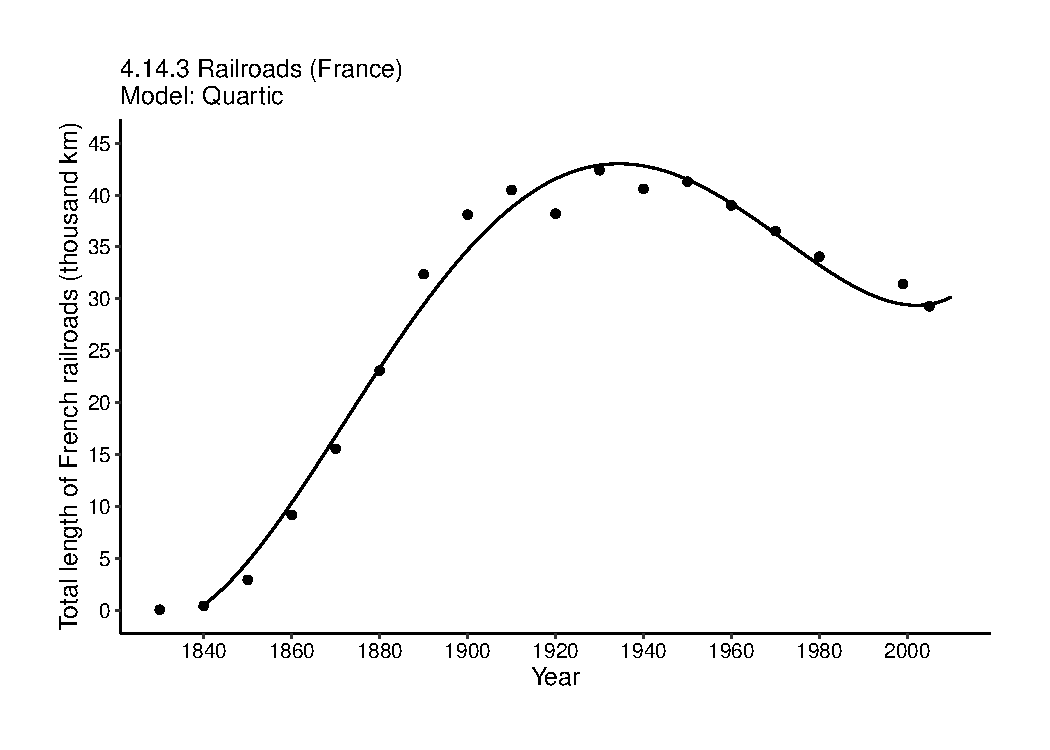
\includegraphics[width=\textwidth]{output/figs-ggplot/4.14.3.pdf}
\caption*{\textbf{Dataset 4.14.3} (p. 263). Growth curves of the total length of railroads in France. Plotted from data in Mitchell (1998).}
\end{figure}
	
\clearpage
\begin{figure}[h]
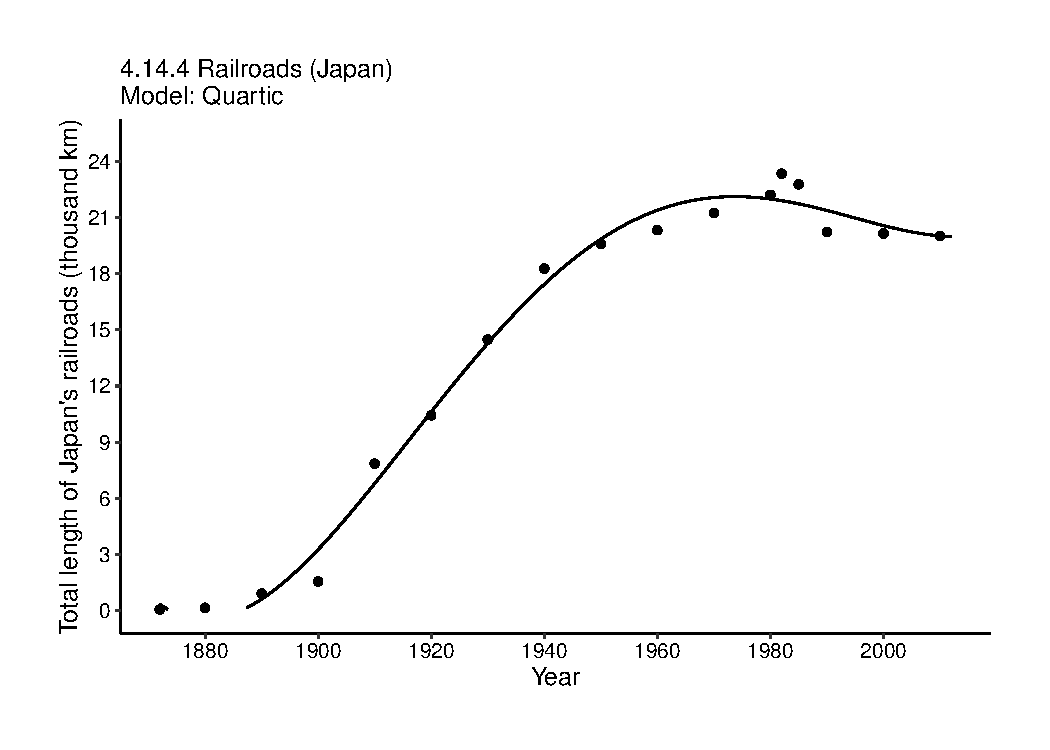
\includegraphics[width=\textwidth]{output/figs-ggplot/4.14.4.pdf}
\caption*{\textbf{Dataset 4.14.4} (p. 263). Growth curves of the total length of railroads in Japan. Plotted from data in Mitchell (1998).}
\end{figure}
	
\clearpage
\begin{figure}[h]
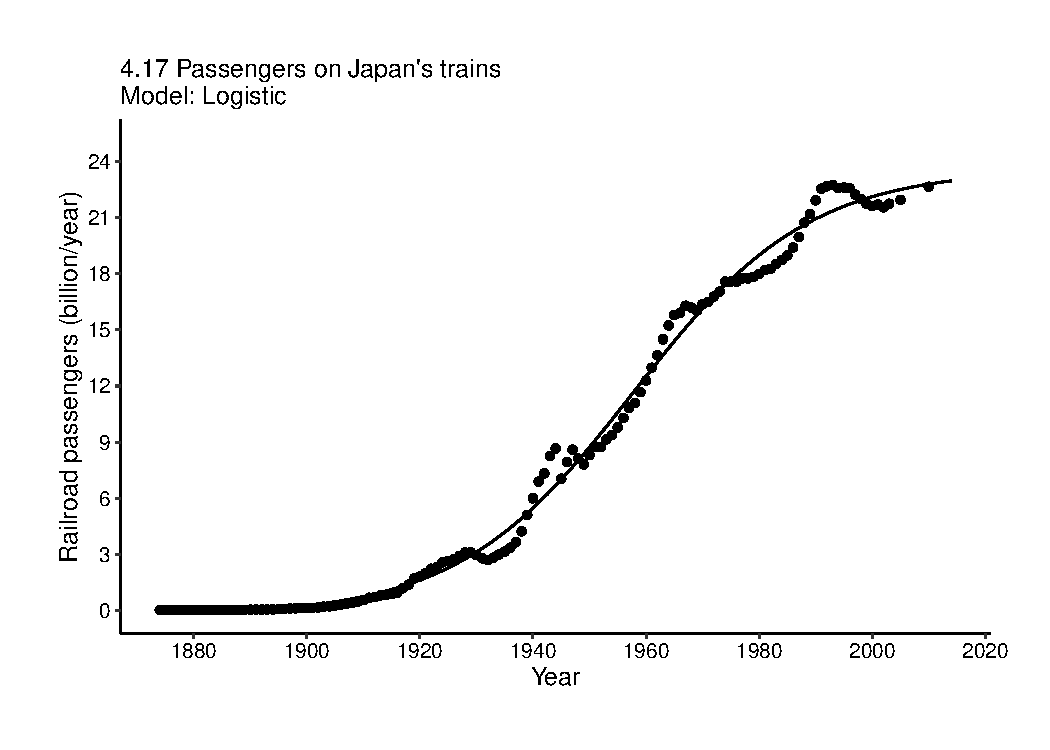
\includegraphics[width=\textwidth]{output/figs-ggplot/4.17.pdf}
\caption*{\textbf{Dataset 4.17} (p. 278). Passengers on Japan's trains, 1874-2014. Plotted from data available at SB (1996, 2017a). Logistic curve with the inflection year in 1958 and with the 2015 total only a fraction of 1 percent below the asymptotic level.}
\end{figure}
	
\clearpage
\begin{figure}[h]
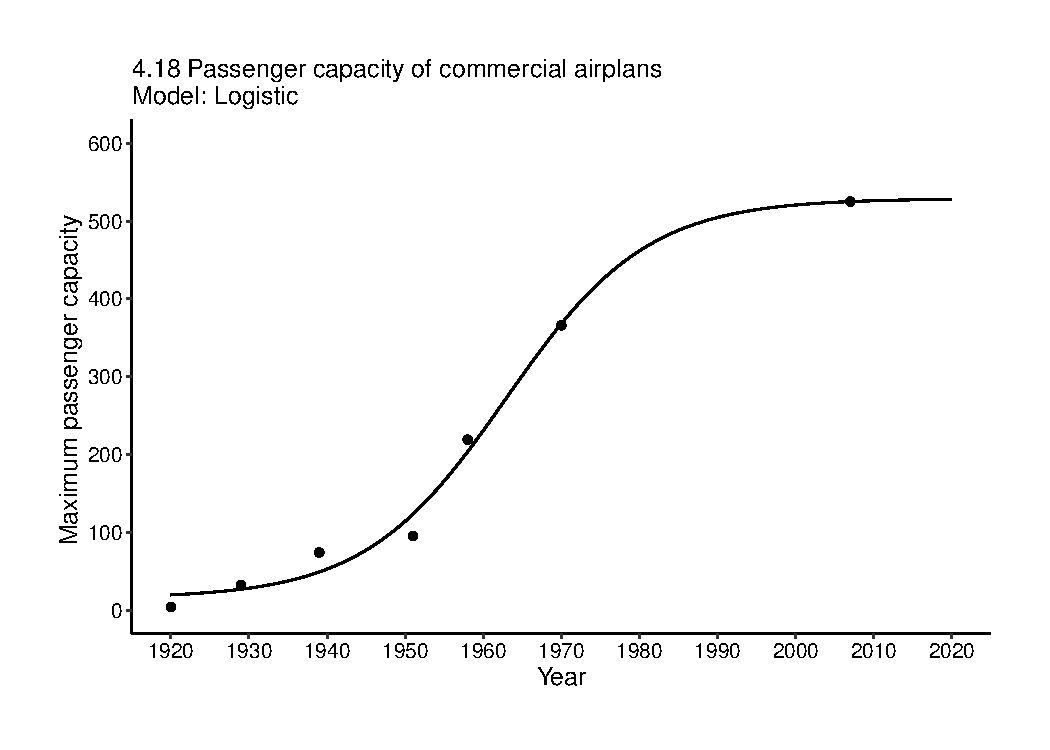
\includegraphics[width=\textwidth]{output/figs-ggplot/4.18.pdf}
\caption*{\textbf{Dataset 4.18} (p. 282). Logistic fit of the maximum passenger capacity of commercial airplans: from KLM's de Havilland DH.16 (four passengers) in 1920 to Airbus 380 (544 passengers in three classes, 868 maximum) in 2007. Plotted from individual airplane specifications.}
\end{figure}
	
\clearpage
\begin{figure}[h]
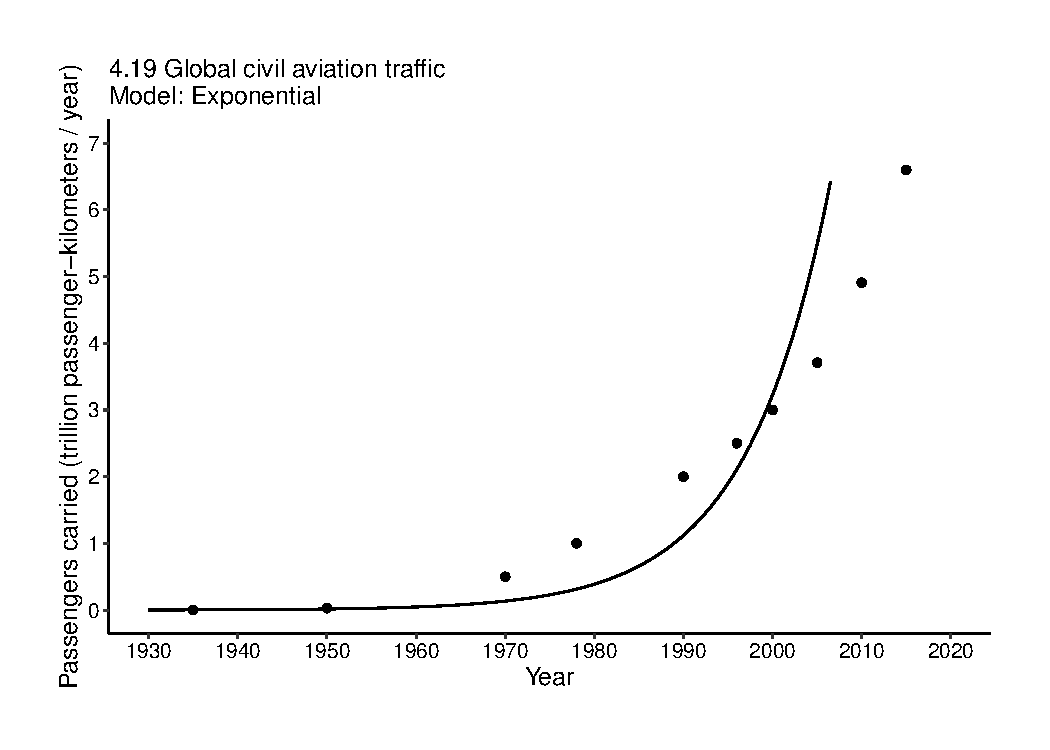
\includegraphics[width=\textwidth]{output/figs-ggplot/4.19.pdf}
\caption*{\textbf{Dataset 4.19} (p. 283). Growth of global civil aviation traffic (domestic and international flights) measured in terms of passenger-kilometers. Logistic curve in its early stage indicates further substantial growth in the decades ahead. Data from ICAO (2016) and from earlier annual reports. }
\end{figure}
	
\clearpage
\begin{figure}[h]
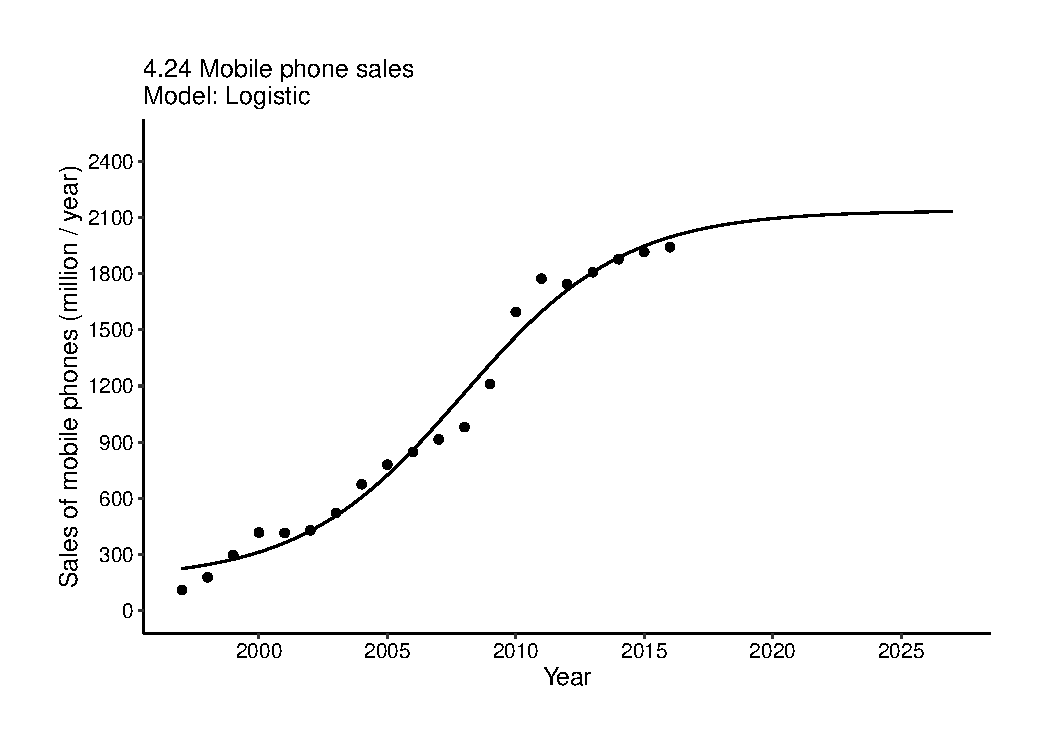
\includegraphics[width=\textwidth]{output/figs-ggplot/4.24.pdf}
\caption*{\textbf{Dataset 4.24} (p. 296). Growth of annual sales of all mobile phones since 1997. The trajectory fits a logistic curve that inflected in 2008 and that is now approaching its asymptotic value. Data from GSMArena (2017).}
\end{figure}
	
\clearpage
\begin{figure}[h]
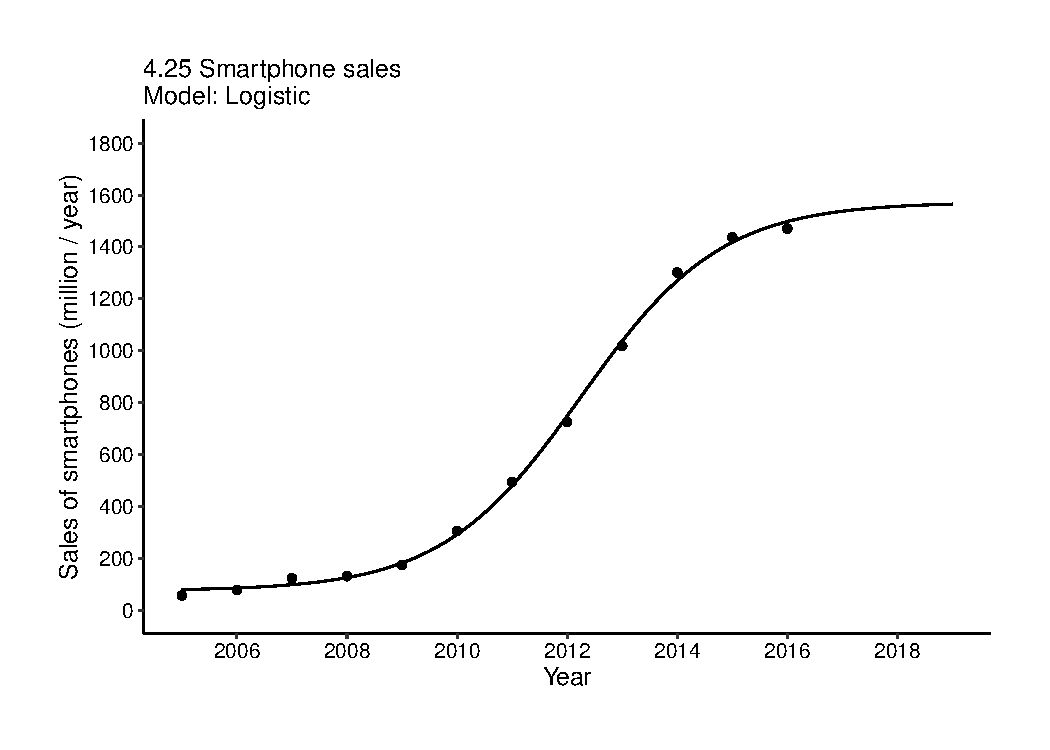
\includegraphics[width=\textwidth]{output/figs-ggplot/4.25.pdf}
\caption*{\textbf{Dataset 4.25} (p. 297). The growth of annual sales of smartphones since the year 2005 has followed perfectly a logistic curve with the inflection year in 2012 and with the asymptote less than 10\% above 2016 sales. Data from Canalys (2007) and Meeker (2017).}
\end{figure}
	
\clearpage
\begin{figure}[h]
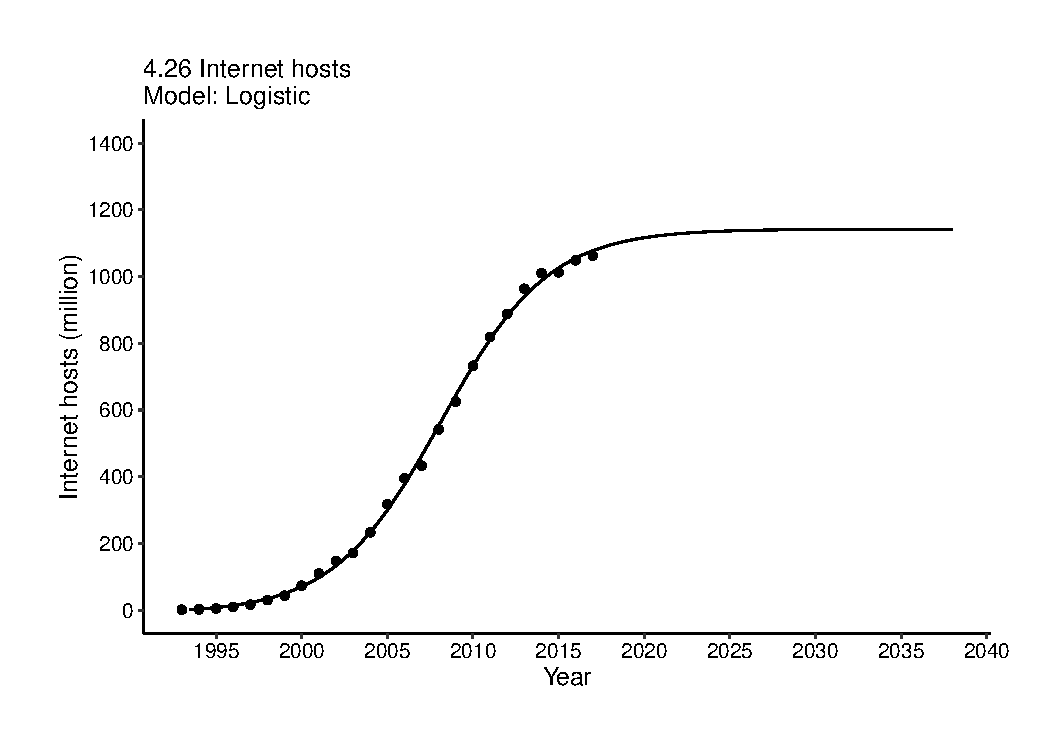
\includegraphics[width=\textwidth]{output/figs-ggplot/4.26.pdf}
\caption*{\textbf{Dataset 4.26} (p. 299). The post-1993 growth of Internet hosts has followed a logistic curve with the inflection year in 2008 and with the asymptotic value less than 10\% above the 2017 total. Data from ISC (2017). }
\end{figure}
	
\clearpage
\begin{figure}[h]
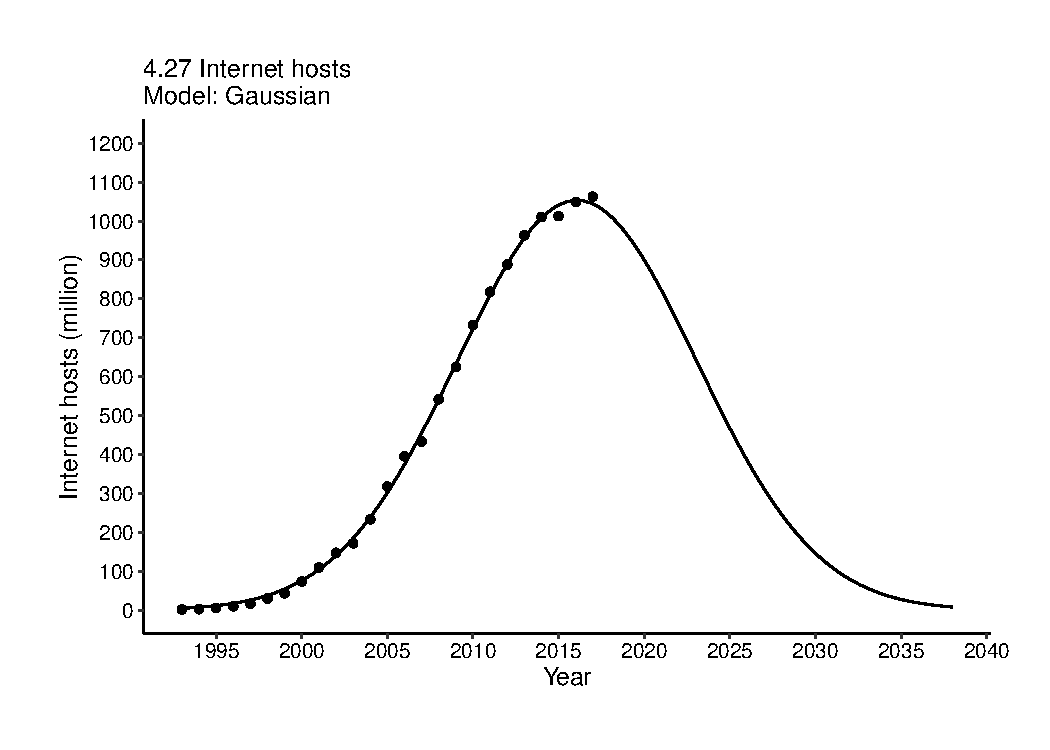
\includegraphics[width=\textwidth]{output/figs-ggplot/4.27.pdf}
\caption*{\textbf{Dataset 4.27} (p. 299). The growth of Internet hosts also fits a Gaussian curve peaking in 2016 and returning to negligible values before 2040. Such a development seems quite unlikely - unless a new mode of hosting takes over. Data from ISC (2017).}
\end{figure}
	
\clearpage
\begin{figure}[h]
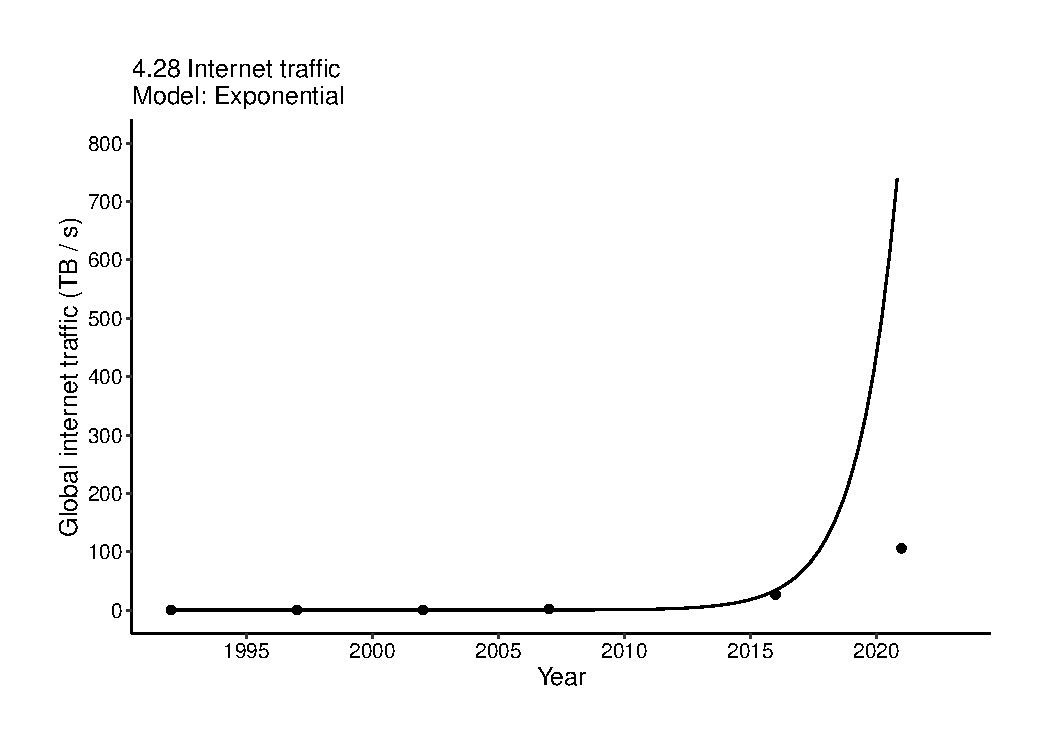
\includegraphics[width=\textwidth]{output/figs-ggplot/4.28.pdf}
\caption*{\textbf{Dataset 4.28} (p. 300). Post-1992 growth of Internet traffic in TB/s fits a logistic curve in its early stages of growth indicating further substantial gains in decades ahead. Data from CISCO (2017).}
\end{figure}
	
\clearpage
\begin{figure}[h]
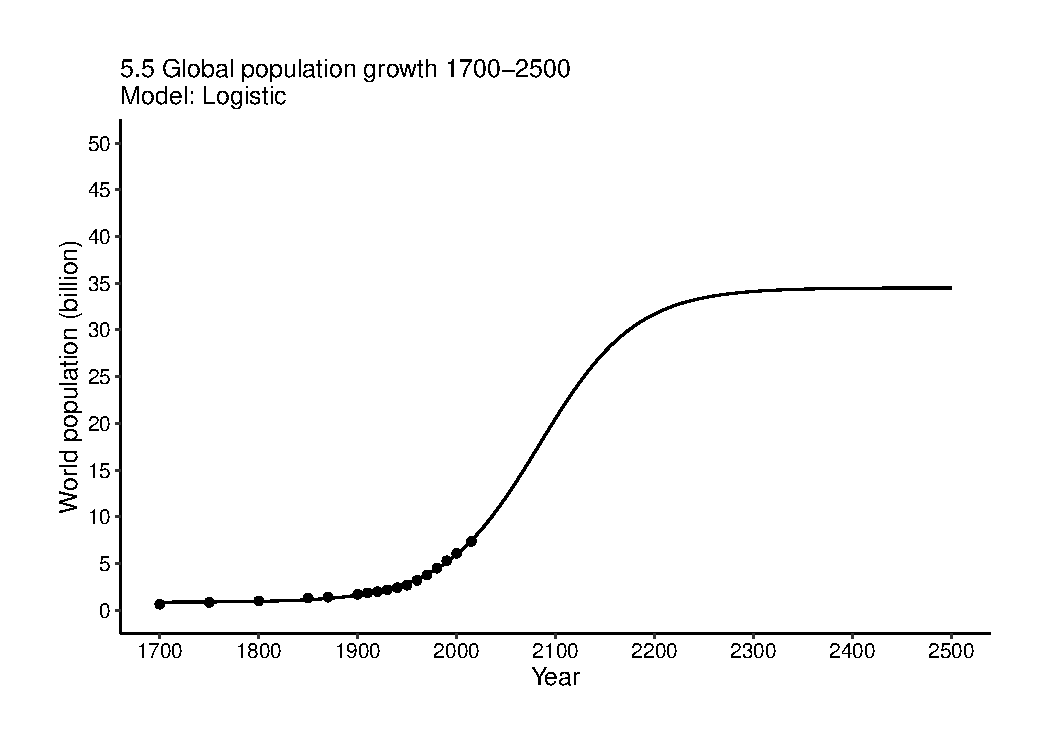
\includegraphics[width=\textwidth]{output/figs-ggplot/5.5.pdf}
\caption*{\textbf{Dataset 5.5} (p. 332). Global population growth, 1700-2500. Logistic curve with a distant inflection point (in 2105) and asymptote of 45.2 billion. }
\end{figure}
	
\clearpage
\begin{figure}[h]
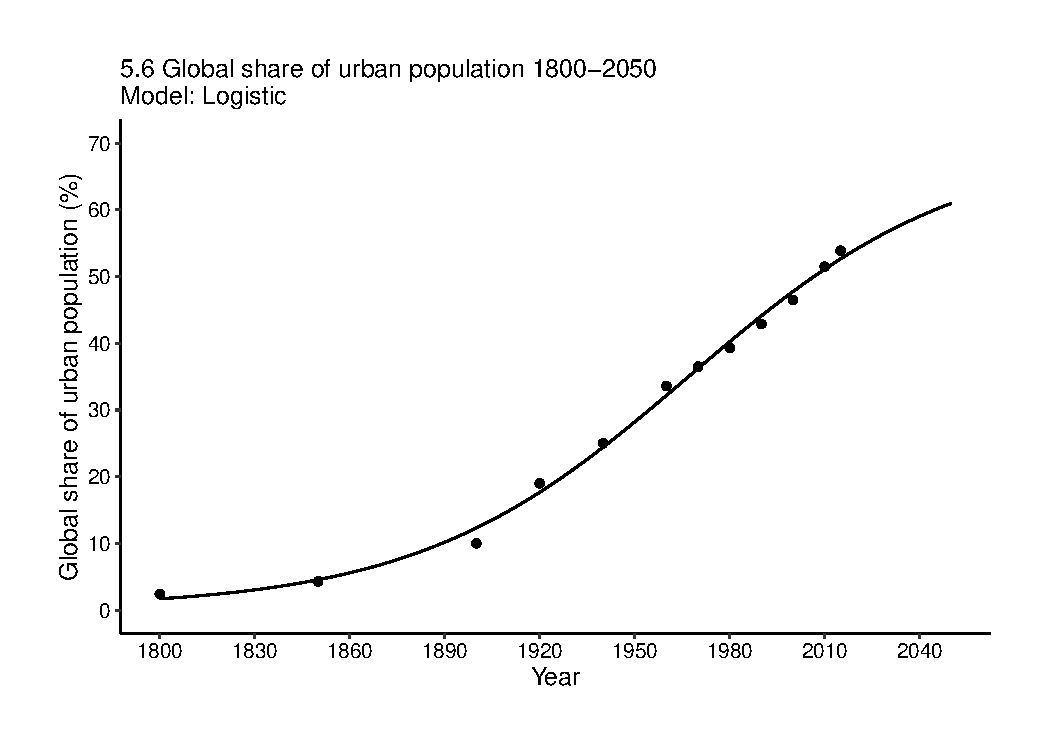
\includegraphics[width=\textwidth]{output/figs-ggplot/5.6.pdf}
\caption*{\textbf{Dataset 5.6} (p. 337). Global share of the urban population, 1800-2050. Plotted from various UN statistics. Logistic curve with the inflection point in 1969 and asymptote of 70.9\%.}
\end{figure}
	
\clearpage
\begin{figure}[h]
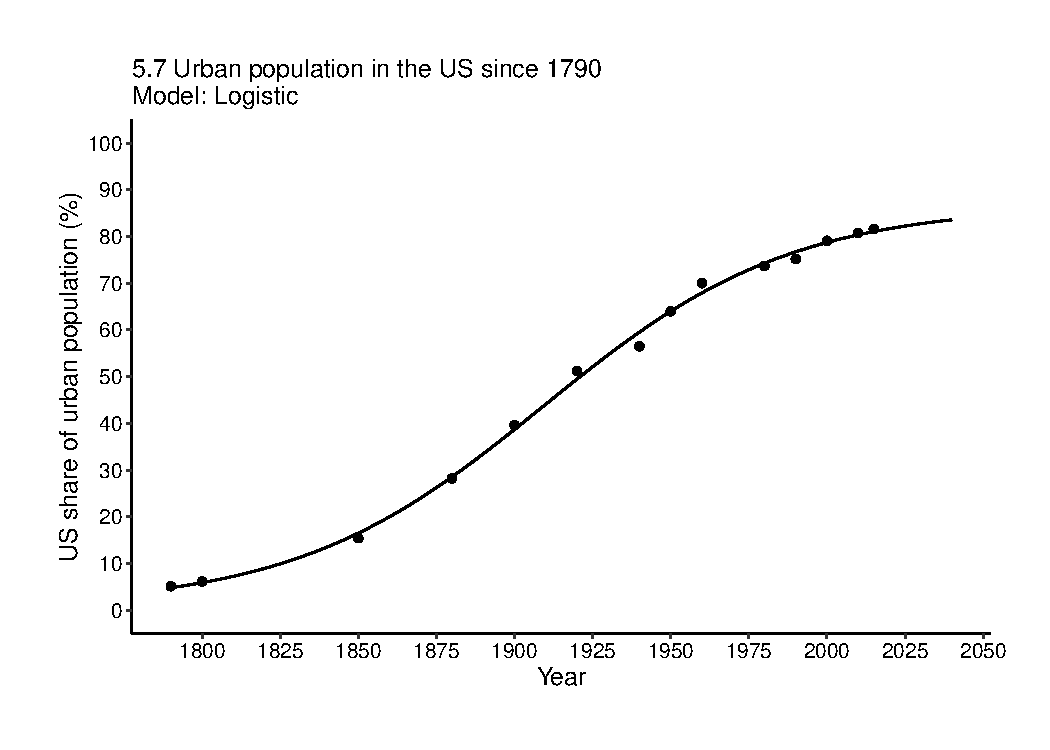
\includegraphics[width=\textwidth]{output/figs-ggplot/5.7.pdf}
\caption*{\textbf{Dataset 5.7} (p. 338). Share of the urban population in the US since 1790. Plotted from data in USBC (1975) and subsequent volumes of US Statistical Abstract. With the logistic curve inflected already in 1910, its asymptotic value is 87.2\%.}
\end{figure}
	
\clearpage
\begin{figure}[h]
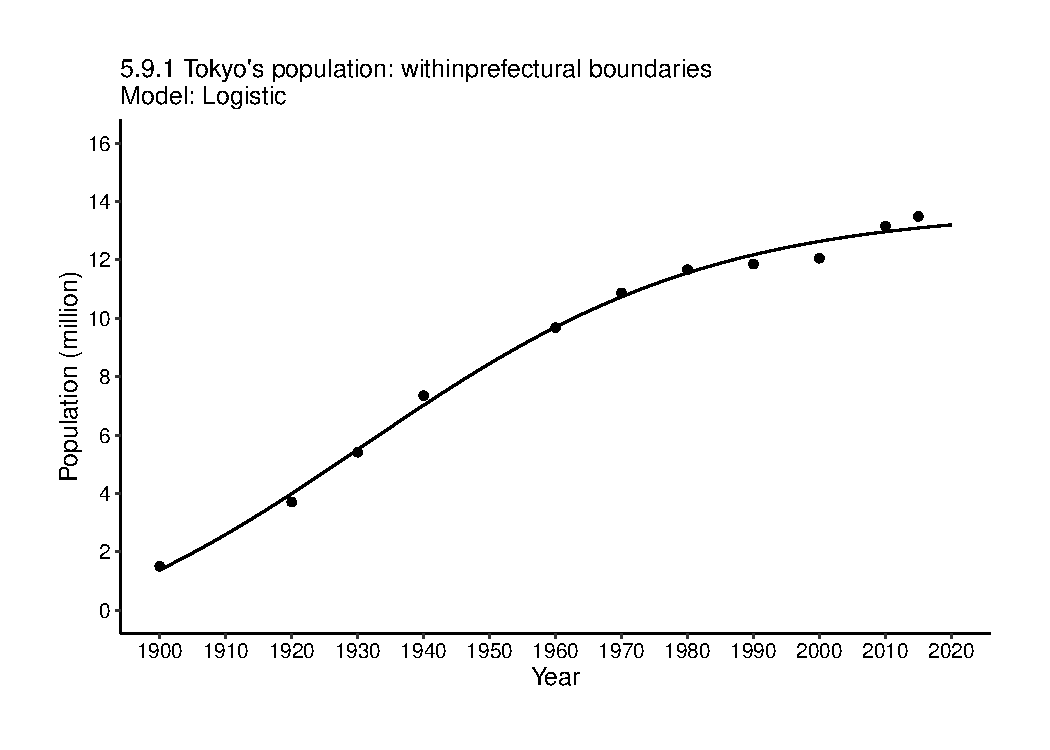
\includegraphics[width=\textwidth]{output/figs-ggplot/5.9.1.pdf}
\caption*{\textbf{Dataset 5.9.1} (p. 349). Tokyo's population within prefectural boundaries (1900-2020) - a logistic curve with the inflection point in 1932 and asymptote at 13.8 million - and within the Tokyo Major Metropolitan Region since 1920: logistic curve infelction point in 1971 and asymptote at 38.8 million. Data from SB (1996) and TMG (2017). }
\end{figure}
	
\clearpage
\begin{figure}[h]
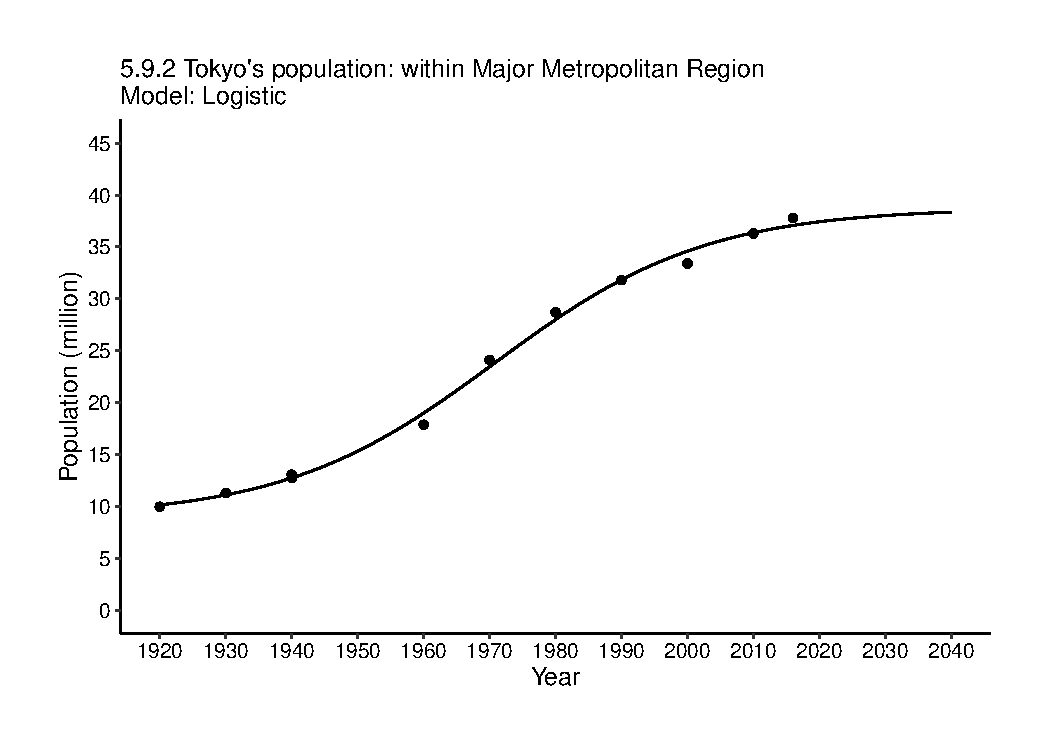
\includegraphics[width=\textwidth]{output/figs-ggplot/5.9.2.pdf}
\caption*{\textbf{Dataset 5.9.2} (p. 349). Tokyo's population within prefectural boundaries (1900-2020) - a logistic curve with the inflection point in 1932 and asymptote at 13.8 million - and within the Tokyo Major Metropolitan Region since 1920: logistic curve infelction point in 1971 and asymptote at 38.8 million. Data from SB (1996) and TMG (2017). }
\end{figure}
	
\clearpage
\begin{figure}[h]
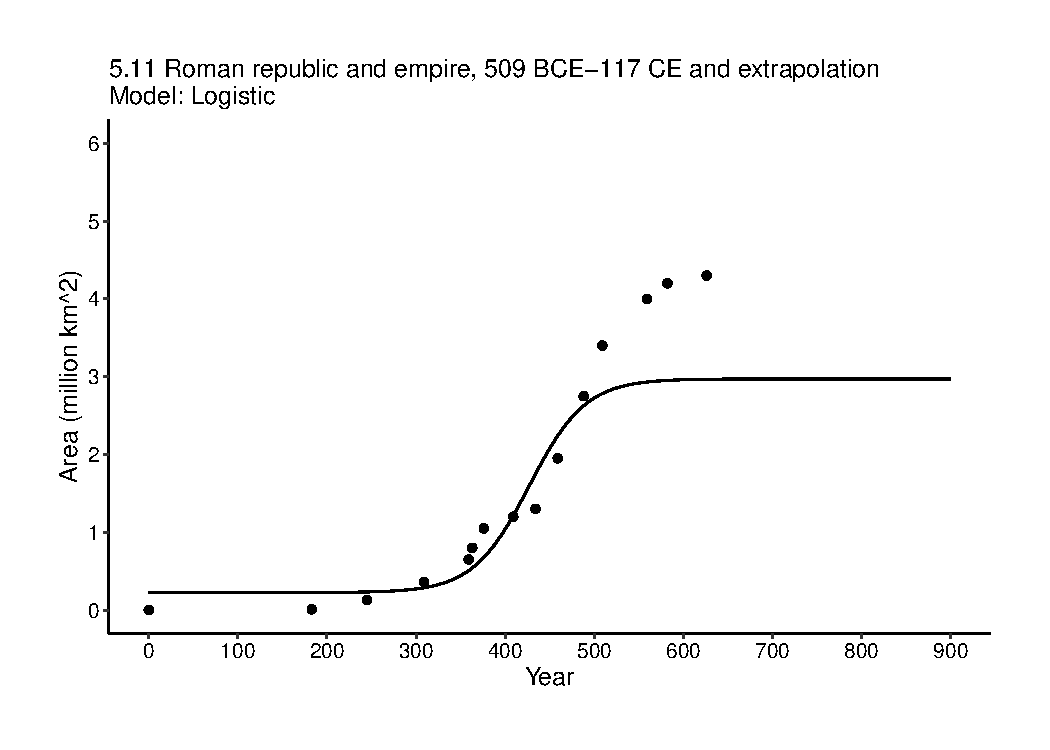
\includegraphics[width=\textwidth]{output/figs-ggplot/5.11.pdf}
\caption*{\textbf{Dataset 5.11} (p. 372). Growth of the Roman republic and empire, 509 BCE-117 CE and the implied future trajectory based on a logistic fit. Data from Taagepera (1979) and author's area measurements based on Talbert (2000). Year zero is 509 BCE. }
\end{figure}
	
\clearpage
\begin{figure}[h]
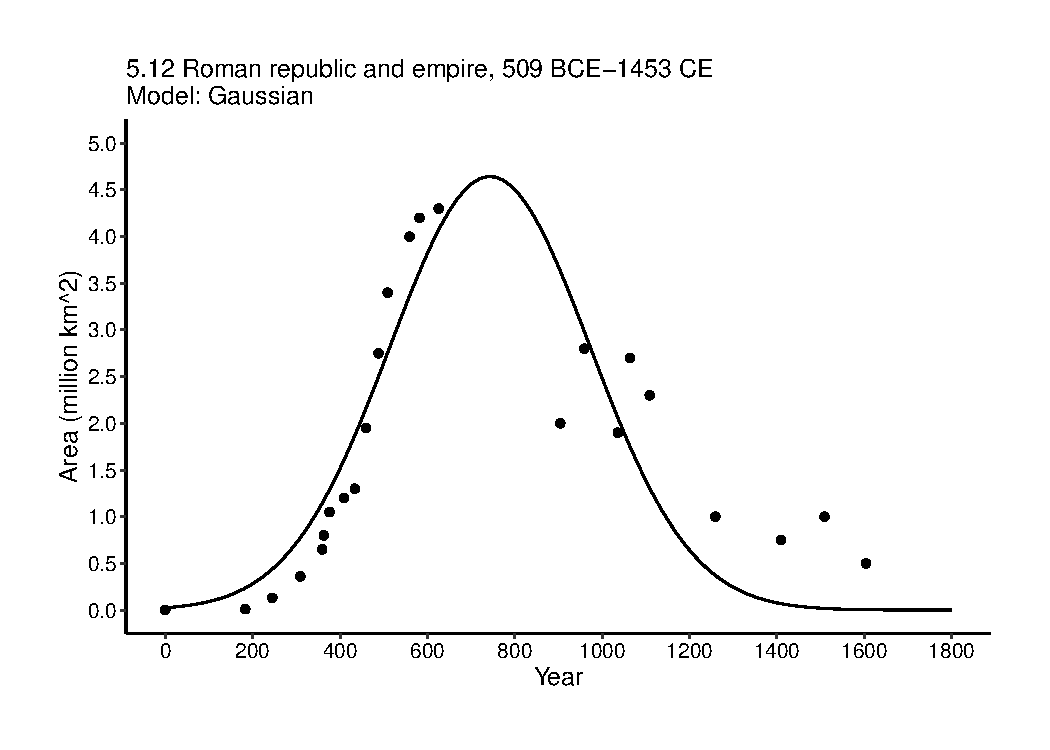
\includegraphics[width=\textwidth]{output/figs-ggplot/5.12.pdf}
\caption*{\textbf{Dataset 5.12} (p. 373). Growth of the Roman republic and empire and the gradual retreat of Byzantium, 509 BCE-1453 CE. Data from Taagepera (1979) and author's area measurements based on Talbert (2000). Year zero is 509 BCE. }
\end{figure}
	
\clearpage
\begin{figure}[h]
\includegraphics[width=\textwidth]{output/figs-ggplot/5.13.1.pdf}
\caption*{\textbf{Dataset 5.13.1} (p. 379). Growth of global primary energy supply (including traditional biomass fuels) and fossil fuel and primary electricity supply since 1800. Data from Smil (2017b). }
\end{figure}
	
\clearpage
\begin{figure}[h]
\includegraphics[width=\textwidth]{output/figs-ggplot/5.13.2.pdf}
\caption*{\textbf{Dataset 5.13.2} (p. 379). Growth of global primary energy supply (including traditional biomass fuels) and fossil fuel and primary electricity supply since 1800. Data from Smil (2017b). }
\end{figure}
	
\clearpage
\begin{figure}[h]
\includegraphics[width=\textwidth]{output/figs-ggplot/5.14.pdf}
\caption*{\textbf{Dataset 5.14} (p. 380). Growth of global crude oil production since 1870. Data from Smil (2017b).}
\end{figure}
	
\clearpage
\begin{figure}[h]
\includegraphics[width=\textwidth]{output/figs-ggplot/5.15.pdf}
\caption*{\textbf{Dataset 5.15} (p. 381). Growth of global natural gas extraction since 1870. Data from Smil (2017b).}
\end{figure}
	
\clearpage
\begin{figure}[h]
\includegraphics[width=\textwidth]{output/figs-ggplot/5.16.pdf}
\caption*{\textbf{Dataset 5.16} (p. 382). Growth of global coal produciton since 1800. While the two logistic curves for crude oil and natural gas provide a highly plausible indication of future development, coal's indicated trajectory will almost certainly diverge from the indicated trend. Data from Smil (2017b). }
\end{figure}
	
\clearpage
\begin{figure}[h]
\includegraphics[width=\textwidth]{output/figs-ggplot/5.17.pdf}
\caption*{\textbf{Dataset 5.17} (p. 383). Growth of global electricity generation since 1900. Data from Smil (2017b) and BP (2017). }
\end{figure}
	
\clearpage
\begin{figure}[h]
\includegraphics[width=\textwidth]{output/figs-ggplot/5.18.pdf}
\caption*{\textbf{Dataset 5.18} (p. 384). Growth of global hydroelectricity generation since 1900. Data from Smil (2017b) and BP (2017).}
\end{figure}
	
\clearpage
\begin{figure}[h]
\includegraphics[width=\textwidth]{output/figs-ggplot/5.19.pdf}
\caption*{\textbf{Dataset 5.19} (p. 385). Growth of global nuclear generation since 1960. Data from Smil (2017b) and BP (2017).}
\end{figure}
	
\clearpage
\begin{figure}[h]
\includegraphics[width=\textwidth]{output/figs-ggplot/5.20.pdf}
\caption*{\textbf{Dataset 5.20} (p. 387). Growth of global cropland, 1700-2050. Logistic curve had its inflection point in 1876 and the total is now less than 5\% below the asymptote. Data from PBL (2010) and FAO (2018).}
\end{figure}
	
\clearpage
\begin{figure}[h]
\includegraphics[width=\textwidth]{output/figs-ggplot/5.21.pdf}
\caption*{\textbf{Dataset 5.21} (p. 387). Growth of US cropland, 1700-2050. Inflection point came already in 1876 and the recently cultivated area is very close to the asymptotic level. Data from PBL (2010) and FAO (2018).}
\end{figure}
	
\clearpage
\begin{figure}[h]
\includegraphics[width=\textwidth]{output/figs-ggplot/5.22.pdf}
\caption*{\textbf{Dataset 5.22} (p. 388). Growth of global grasslands. The inflection year was in 1923 and the total area is now less than 10\% from the asymptotic level. Data from PBL (2010) and FAO (2018).}
\end{figure}
	
\clearpage
\begin{figure}[h]
\includegraphics[width=\textwidth]{output/figs-ggplot/5.23.pdf}
\caption*{\textbf{Dataset 5.23} (p. 390). Worldwide production of nitrogenous fertilizers since 1913. Another logistic curve that is very close to its asymptote. Data from Smil (2001) and FAO (2018).}
\end{figure}
	
\clearpage
\begin{figure}[h]
\includegraphics[width=\textwidth]{output/figs-ggplot/5.24.pdf}
\caption*{\textbf{Dataset 5.24} (p. 391). Global harvest of staple grain crops since 1900. Data from Smil (2013a) and FAO (2018).}
\end{figure}
	
\clearpage
\begin{figure}[h]
\includegraphics[width=\textwidth]{output/figs-ggplot/5.28.pdf}
\caption*{\textbf{Dataset 5.28} (p. 398). Logistic curve of worldwide semiconductor sales, 1976-2016. Plotted from data in SIA (2017).}
\end{figure}
	
\clearpage
\begin{figure}[h]
\includegraphics[width=\textwidth]{output/figs-ggplot/5.29.1.pdf}
\caption*{\textbf{Dataset 5.29.1} (p. 412). Growth and logistic outlook of GDP (expression in international \$2011) in four major economies - France, Japan, and the US since 1870, and China since 1950. Data from World Bank (2018).}
\end{figure}
	
\clearpage
\begin{figure}[h]
\includegraphics[width=\textwidth]{output/figs-ggplot/5.29.2.pdf}
\caption*{\textbf{Dataset 5.29.2} (p. 412). Growth and logistic outlook of GDP (expression in international \$2011) in four major economies - France, Japan, and the US since 1870, and China since 1950. Data from World Bank (2018).}
\end{figure}
	
\clearpage
\begin{figure}[h]
\includegraphics[width=\textwidth]{output/figs-ggplot/5.29.3.pdf}
\caption*{\textbf{Dataset 5.29.3} (p. 412). Growth and logistic outlook of GDP (expression in international \$2011) in four major economies - France, Japan, and the US since 1870, and China since 1950. Data from World Bank (2018).}
\end{figure}
	
\clearpage
\begin{figure}[h]
\includegraphics[width=\textwidth]{output/figs-ggplot/5.29.4.pdf}
\caption*{\textbf{Dataset 5.29.4} (p. 412). Growth and logistic outlook of GDP (expression in international \$2011) in four major economies - France, Japan, and the US since 1870, and China since 1950. Data from World Bank (2018).}
\end{figure}
	
\clearpage
\begin{figure}[h]
\includegraphics[width=\textwidth]{output/figs-ggplot/5.30.1.pdf}
\caption*{\textbf{Dataset 5.30.1} (p. 418). Growth of per capita income in the US, Japan, and China since 1950. Data from World Bank (2018).}
\end{figure}
	
\clearpage
\begin{figure}[h]
\includegraphics[width=\textwidth]{output/figs-ggplot/5.30.2.pdf}
\caption*{\textbf{Dataset 5.30.2} (p. 418). Growth of per capita income in the US, Japan, and China since 1950. Data from World Bank (2018).}
\end{figure}
	
\clearpage
\begin{figure}[h]
\includegraphics[width=\textwidth]{output/figs-ggplot/5.30.3.pdf}
\caption*{\textbf{Dataset 5.30.3} (p. 418). Growth of per capita income in the US, Japan, and China since 1950. Data from World Bank (2018).}
\end{figure}
	
\clearpage
\begin{figure}[h]
\includegraphics[width=\textwidth]{output/figs-ggplot/5.31.pdf}
\caption*{\textbf{Dataset 5.31} (p. 431). Growing shares of international trade in the world economic product since 1870. Data from Klasing and Milionis (2014) and World Bank (2018).}
\end{figure}
	
\clearpage
\begin{figure}[h]
\includegraphics[width=\textwidth]{output/figs-ggplot/6.1.pdf}
\caption*{\textbf{Dataset 6.1} (p. 452). US crude oil extraction forecast based on the 1900-1980 trajectory. Data from USBC (1975) and USEIA (2019). }
\end{figure}
	
\clearpage
\begin{figure}[h]
\includegraphics[width=\textwidth]{output/figs-ggplot/6.2.1.pdf}
\caption*{\textbf{Dataset 6.2.1} (p. 453). Population of Greater London: best fits based on 1801-1981 (a) and 1801-2001 (b) totals. Data from Morrey (1978) and GLA (2015). }
\end{figure}
	
\clearpage
\begin{figure}[h]
\includegraphics[width=\textwidth]{output/figs-ggplot/6.2.2.pdf}
\caption*{\textbf{Dataset 6.2.2} (p. 453). Population of Greater London: best fits based on 1801-1981 (a) and 1801-2001 (b) totals. Data from Morrey (1978) and GLA (2015). }
\end{figure}
	
\clearpage
\begin{figure}[h]
\includegraphics[width=\textwidth]{output/figs-ggplot/6.7.pdf}
\caption*{\textbf{Dataset 6.7} (p. 464). British steel output, 1900-2020. Fluctuating output reflects economic downturns, expansions, and wars and hence the normal curve is not a particularly close fit ($R^2$ of 0.79). The production peak came in1970, with the 2015 output below the level attained first in 1936. Data from https://visual.ons.gov.uk/the-british-steel-industry-since-the-1970s}
\end{figure}
	
\clearpage
\begin{figure}[h]
\includegraphics[width=\textwidth]{output/figs-ggplot/6.9.pdf}
\caption*{\textbf{Dataset 6.9} (p. 466). Number of American draft horses between 1850 and 1970 conforms closely to the normal curve trajectory. Data from USBC (1975). }
\end{figure}
	
\clearpage
\begin{figure}[h]
\includegraphics[width=\textwidth]{output/figs-ggplot/6.10.pdf}
\caption*{\textbf{Dataset 6.10} (p. 467). Number of US steam locomotives: a very good Gaussian fit for the nine decades between 1876 and 1967. Data from USBC (1975). }
\end{figure}
	
\clearpage
\begin{figure}[h]
\includegraphics[width=\textwidth]{output/figs-ggplot/6.11.pdf}
\caption*{\textbf{Dataset 6.11} (p. 467). The historical growth of the US passenger car fleet can be fitted quite well into a normal curve peaking around 2030. Data from USBC (1975) and from subsequent volumes of the US Statistical Abstract. }
\end{figure}
	
\section*{Bibliography}

This bibliography is taken directly from Smil (2019). References appear exactly as they do there (minus some formatting). \par\par

BP (British Petroleum). 2017. BP Statistical Review of World Energy. London: BP.\par
Ballal, D., and J. Zelina. 2003. Progress in aeroengine technology (1939–2003). Journal of Aircraft 41:43–50.\par
Beaver, P. 1972. A History of Tunnels. Secaucus, NJ: Citadel Press.\par
Buchanan, R. L., et al. 1997. When is simple good enough: A comparison of the Gompertz, Baranyi, and three-phase models for fitting bacterial growth curves. Food Microbiology 14:313–326.\par
CISCO. 2017. The zettabyte era: Trends and analysis. \url{https://webobjects.cdw.com/webobjects/media/pdf/Solutions/Networking/White-Paper-Cisco-The-Zettabyte-Era-Trends-and-Analysis.pdf}.\par
Canalys. 2007. 64 million smart phones shipped worldwide in 2006. \url{https://www.canalys.com/static/press_release/2007/r2007024.pdf}.\par
Daugherty, C. R. 1927. The development of horse-power equipment in the United States. In C. R. Daugherty et al., Power Capacity and Production in the United States. Washington, DC: US Geological Survey, pp. 5–112.\par
Emporis. 2017. Cities with most skyscrapers. \url{https://www.emporis.com/statistics/most-skyscraper-cities-worldwide}.\par
FAO. 2018. Faostat. \url{http://www.fao.org/faostat/en/#data}.\par
GLA (Greater London Authority). 2015. Population Growth in London, 1939–2015. London: GLA.\par
GSMArena. 2017. All mobile phone brands. \url{http://www.gsmarena.com/makers.php3}.\par
Giegling, F., et al., eds. 1964. Chronologisch-thematisches Verzeichnis sämtlicher Tonwerke Wolfgang Amade Mozarts. Wiesbaden: Breitkopf \& Härtel.\par
History of Bridges. 2017. The world’s longest bridge—Danyang–Kunshan Grand Bridge. \url{http://www.historyofbridges.com/famous-bridges/longest-bridge-in-the-world/}.\par
ICAO (International Civil Aviation Organization). 2016. Annual Report 2016. \url{https://www.icao.int/annual-report-2016/Pages/default.aspx}.\par
ICOLD (International Commission on Large Dams). 2017. World Register of Dams. \url{http://www.icold-cigb.net/GB/world_register/world_register_of_dams.asp}.\par
ISC (Internet System Consortium). 2017. ISC Internet domain survey. \url{https://www.isc.org/network/survey/}.\par
Klasing, M. J., and P. Milionis. 2014. Quantifying the evolution of world trade, 1870–1949. Journal of International Economics 92:185–197.\par
Landau, S. B., and C. W. Condit. 1996. Rise of the New York Skyscraper, 1865–1913. New Haven, CT: Yale University Press.\par
Meeker, M. 2017. Internet trends 2017—code conference. \url{http://www.kpcb.com/internet-trends}.\par
Mitchell, B., ed. 1998. International Historical Statistics. London: Palgrave Macmillan.\par
Morrey, C. R. 1978. The Changing Population of the London Boroughs. London: Greater London Council.\par
NBS (National Bureau of Statistics of China). 2000. China Statistical Yearbook 2000. Beijing: NBS.\par
NBS. 2016. China Statistical Yearbook 2016. Beijing: NBS. \url{http://www.stats.gov.cn/tjsj/ndsj/2016/indexeh.htm}.\par
Onoda, S. 2015. Tunnels in Japan. Japan Railway \& Transport Review 66:38–51.\par
PBL (Planbureau voor de Leefomgeving). 2010. Land use data. \url{http://themasites.pbl.nl/tridion/en/themasites/hyde/landusedata/index-2.html}.\par
Pearl, R., and L. J. Reed. 1920. On the rate of growth of the population of the United States since 1790 and its mathematical representation. Proceedings of the National Academy of Sciences of the USA 6:275–288.\par
Reed, H. S., and R. H. Holland. 1919. The growth rate of an annual plant Helianthus. Proceedings of the National Academy of Sciences of the USA 5:135–144.\par
SB (Statistics Bureau, Japan). 1996. Historical Statistics of Japan. \url{http://www.stat.go.jp/english/data/chouki/}.\par
SB. 2017a. Japan Statistical Yearbook. Tokyo: SB. \url{http://www.stat.go.jp/english/data/handbook/pdf/2017all.pdf}.\par
SIA (Semiconductor Industry Association). 2017. 2017 Factbook. \url{http://go.semiconductors.org/2017-sia-factbook-0-0-0}.\par
Schurr, S. H., and B. C. Netschert. 1960. Energy in the American Economy 1850–1975. Baltimore, MD: Johns Hopkins University Press.\par
Schurr, S. H., et al. 1990. Electricity in the American Economy: Agent of Technological Progress. New York: Greenwood Press.\par
Skyscraper Center. 2017. 100 tallest completed buildings in the world by height to architectural top. \url{https://www.skyscrapercenter.com/buildings}.\par
Smil, V. 2001. Enriching the Earth. Cambridge, MA: MIT Press.\par
Smil, V. 2003. Energy at the Crossroads. Cambridge, MA: MIT Press.\par
Smil, V. 2008. Energy in Nature and Society. Cambridge, MA: MIT Press.\par
Smil, V. 2010b. Prime Movers of Globalization. Cambridge, MA: MIT Press.\par
Smil, V. 2013a. Harvesting the Biosphere. Cambridge, MA: MIT Press.\par
Smil, V. 2014b. Making the Modern World. Chichester: Wiley.\par
Smil, V. 2017a. Energy and Civilization. Cambridge, MA: MIT Press.\par
Smil, V. 2017b. Energy Transitions. Santa Barbara, CA: Praeger.\par
TMG (Tokyo Metropolitan Region). 2017. The structure of the Tokyo Metropolitan Government (TMG). \url{http://www.metro.tokyo.jp/ENGLISH/ABOUT/STRUCTURE/structure02.htm}.\par
Taagepera, R. 1978. Size and duration of empires: Growth-decline curves, 3000 to 600 B.C. Social Science Research 7:180–196.\par
Talbert, R. J. A., ed. 2000. Barrington Atlas of the Greek and Roman World. Princeton, NJ: Princeton University Press.\par
The State of Obesity. 2017. Adult obesity in the United States. \url{http://stateofobesity.org/adult-obesity/}.\par
USBC (United States Bureau of the Census). 1975. Historical Statistics of the United States: Colonial Times to 1970. Washington, DC: USBC.\par
USCB. 2016a. Highlights of annual 2015 characteristics of new housing. \url{https://www.census.gov/construction/chars/highlights.html}.\par
USDA. 2017a. Crop production historical track records. \url{http://usda.mannlib.cornell.edu/MannUsda/viewDocumentInfo.do?documentID​=​1593}.\par
USEIA. 2016. Average operating heat rate for selected energy sources. \url{https://www.eia.gov/electricity/annual/html/epa_08_01.html}.\par
USEIA. 2019. U.S. Field Production of Crude Oil. \url{https://www.eia.gov/dnav/pet/hist/LeafHandler.ashx?n​=P​ET&s​=M​ CRFPUS1&f​=​M}.\par
USEPA. 2016b. Light-Duty Vehicle CO2 and Fuel Economy Trends. Washington, DC: USEPA. \url{https://www.epa.gov/fuel-economy-trends/report-tables-and-appendices-co2-and-fuel-economy-trends}.\par
Wilson, A., and J. Boehland. 2005. Small is beautiful: U.S. house size, resource use, and the environment. Journal of Industrial Ecology 9:277–287.\par
World Bank. 2018. DataBank. \url{http://databank.worldbank.org/data/home.aspx}.\par
Zeller, T. 2007. Driving Germany: The Landscape of the German Autobahn, 1930–1970. New York: Berghahn.\par
Zu, C., and H. Li. 2011. Thermodynamic analysis on energy densities of batteries. Energy and Environmental Science 4:2614–2625.\par
\end{document}
